\documentclass{article}
\usepackage[margin=2cm]{geometry}
\usepackage{natbib}
\usepackage{hyperref}
\usepackage{enumitem}
\usepackage{tikz}
\usetikzlibrary{arrows.meta}
\usetikzlibrary{positioning}

\setlist{nosep} % to reduce space in lists

\setlength{\parskip}{0.5em}
\setlength{\parindent}{0in}

%%%%% NEW MATH DEFINITIONS %%%%%
\usepackage{amsmath,bbm,bm}
\usepackage{amssymb}
\usepackage{amsfonts}
\usepackage{amsthm}
\usepackage{mathtools}

% commands
% global count (no section number)
\newtheorem{thm}{Theorem}%[section]
\newtheorem{lem}{Lemma}
\newtheorem{prop}{Proposition}
\newtheorem{cor}{Corollary}
\newtheorem{conj}{Conjecture}
\newtheorem{aspt}{Assumption}
\newtheorem{claim}{Claim}
\newtheorem{rmk}{Remark}
\newtheorem{commt}{Comment}
\newtheorem{defn}{Definition}

% algorithm
%\usepackage{algorithm, algorithmic}
%\usepackage{algorithm2e}
\usepackage{tabularx}
%\usepackage[table,xcdraw]{xcolor}

% Comments
% \usepackage{xcolor} % already loaded
\newcount\comments  % 0 suppresses notes to selves in text
\comments=1  % TODO: change to 0 for final version
\newcommand{\genComment}[2]{\ifnum\comments=1{\textcolor{#1}{\textsf{\footnotesize #2}}}\fi}
\newcommand{\ed}[1]{\genComment{red}{[EI:#1]}}
\newcommand{\giles}[1]{\genComment{green}{[GH:#1]}}
\newcommand{\kevin}[1]{\genComment{blue}{[KT:#1]}}


% Mark sections of captions for referring to divisions of figures
\newcommand{\figleft}{{\em (Left)}}
\newcommand{\figcenter}{{\em (Center)}}
\newcommand{\figright}{{\em (Right)}}
\newcommand{\figtop}{{\em (Top)}}
\newcommand{\figbottom}{{\em (Bottom)}}
\newcommand{\captiona}{{\em (a)}}
\newcommand{\captionb}{{\em (b)}}
\newcommand{\captionc}{{\em (c)}}
\newcommand{\captiond}{{\em (d)}}


\newcommand\seq[2]{{#1}\!:\!{#2}}
\newcommand\R{\mathbb{R}}
\newcommand\Var{\mathrm{Var}}
\newcommand\var{\Var}
\newcommand\Cov{\mathrm{Cov}}
\newcommand\cov{\Cov}
\newcommand\iid{\mathrm{iid}}
\newcommand\dist{d}
\newcommand\lik{\mathcal{L}}
\newcommand\prob{\mathbb{P}}
\newcommand\E{\mathbb{E}}
\newcommand\loglik{\ell}
\newcommand\process{\texttt{process}}
\newcommand\dimtheta{\mathrm{dim}_{\Theta}}
\newcommand\param{\,;}
\newcommand\giventh\param
\newcommand\given{{\,\vert\,}}
\newcommand\code[1]{\texttt{#1}}
\newcommand\ceil[1]{\lceil #1 \rceil}
\newcommand\floor[1]{\lfloor #1 \rfloor}
\newcommand\1{\bm{1}}


% Highlight a newly defined term
\newcommand{\newterm}[1]{{\bf #1}}


% Figure reference, lower-case.
\def\figref#1{figure~\ref{#1}}
% Figure reference, capital. For start of sentence
\def\Figref#1{Figure~\ref{#1}}
\def\twofigref#1#2{figures \ref{#1} and \ref{#2}}
\def\quadfigref#1#2#3#4{figures \ref{#1}, \ref{#2}, \ref{#3} and \ref{#4}}
% Section reference, lower-case.
\def\secref#1{section~\ref{#1}}
% Section reference, capital.
\def\Secref#1{Section~\ref{#1}}
% Reference to two sections.
\def\twosecrefs#1#2{sections \ref{#1} and \ref{#2}}
% Reference to three sections.
\def\secrefs#1#2#3{sections \ref{#1}, \ref{#2} and \ref{#3}}
% Reference to an equation, lower-case.
\def\eqref#1{equation~\ref{#1}}
% Reference to an equation, upper case
\def\Eqref#1{Equation~\ref{#1}}
% A raw reference to an equation---avoid using if possible
\def\plaineqref#1{\ref{#1}}
% Reference to a chapter, lower-case.
\def\chapref#1{chapter~\ref{#1}}
% Reference to an equation, upper case.
\def\Chapref#1{Chapter~\ref{#1}}
% Reference to a range of chapters
\def\rangechapref#1#2{chapters\ref{#1}--\ref{#2}}
% % Reference to an algorithm, lower-case.
% \def\algref#1{algorithm~\ref{#1}}
% % Reference to an algorithm, upper case.
% \def\Algref#1{Algorithm~\ref{#1}}
% \def\twoalgref#1#2{algorithms \ref{#1} and \ref{#2}}
% \def\Twoalgref#1#2{Algorithms \ref{#1} and \ref{#2}}
% Reference to a part, lower case
\def\partref#1{part~\ref{#1}}
% Reference to a part, upper case
\def\Partref#1{Part~\ref{#1}}
\def\twopartref#1#2{parts \ref{#1} and \ref{#2}}

\def\eps{{\epsilon}}

\def\gN{{\mathcal{N}}}
\def\gX{{\mathcal{X}}}
\def\gY{{\mathcal{Y}}}




\newcommand{\off}{\operatorname{off}}
\newcommand{\on}{\operatorname{on}}

\title{Accelerated Inference for Partially Observed Stochastic Processes via Automatic Differentiation}
\author{Kevin Tan}
\date{}

\comments=1

\begin{document}

\maketitle

\begin{center}
    Under the supervision of Giles J. Hooker and Edward L. Ionides
\end{center}

\section{Introduction}



Modeling a stochastic dynamical system in the presence of noisy observations is a challenging problem. Here, likelihood functions are intractable. One can bypass this issue with the approaches of simulated likelihood, likelihood-free inference, and the particle filter, but the Monte Carlo noise in the likelihood estimate that these approaches often suffer from makes parameter estimation difficult. Furthermore, many scientific applications, such as in disease modeling, deal with models where transition densities of the underlying stochastic process are unavailable. Existing statistical workhorses such as the EM algorithm, the Kalman filter, or MCMC, either struggle with intractable likelihoods or assume access to transition densities.

Still, all is not lost. A specific variant (the bootstrap filter) of the particle filter, a popular method for solving the filtering problem in partially-observed dynamical systems, does not require transition densities. Instead, one only requires access to a simulator instead. This provides an unbiased estimate of the likelihood \citep{delmoral2004feynman} that can be used for parameter estimation.

\subsection{Existing Algorithms}

Currently, only three full-information simulation-based algorithms exist for parameter estimation: improved iterated filtering (IF2) \citep{ionides15}, particle MCMC \citep{doucet2010pmcmc}, and SMC$^2$ \citep{chopin13}. Only the first is frequentist, while the other two are Bayesian. 

Here, we will focus on maximum likelihood inference for partially observed Markov processes, and as such we provide a brief outline of IF2. IF2 augment the state space by assigning each particle $x_{n,j}$ its own set of parameters $\theta_{n,j}$. The parameters thought of as latent states that evolve according to Brownian motion on the parameter space $\Theta$. This yields a Monte Carlo approximation to the (extended) filtering distribution $f_{\theta_n,X_n|Y_{1:n}}(\theta_{n,j},x_{n,j}^F|y_{1:n}^*)$, given a Gaussian random walk prior on $\theta_{n,j} \sim \gN(\theta_{n-1,j},\sigma^2)$. Repeating the procedure again and again, while shrinking $\sigma^2$, yields convergence of the parameter swarm $\theta_{n,j}^{(m)}$ to the MLE. 

Still, this is not a silver bullet. Though in practice the algorithm of \citet{ionides15} converges quickly to a neighborhood of the MLE, it often struggles to successfully optimize the last few-units of the log-likelihood, as we see below in Figure \ref{fig:if2fail}.

\begin{figure}[htbp!]
    \centering
    \includegraphics[scale=0.5]{imgs/095/if2fail.png}
    \caption{Failure of iterated filtering on maximum likelihood estimation in the Dhaka cholera model of \cite{king08}. IF2 was run 100 times (with the 0th and 80th quantiles represented with the shaded area), but no run finds the MLE. The best run is about 7.5 log-likelihood units short. }
    \label{fig:if2fail}
\end{figure}

\subsection{Is Automatic Differentiation the Answer?}

The original iterated filtering algorithm of \cite{ionides06-pnas} amounts to gradient descent on a noisy particle approximation of the score. Similar particle approximations exist, such as that of \cite{poyiadjis11}, who provide a linear-time estimator with variance quadratic in the length of the trajectory that is consistent for the score. 

It has been shown by \cite{scibior21} that one can recover the asymptotically biased but low variance estimator of \cite{blei2018vsmc} and the consistent but high variance estimator of \cite{poyiadjis11} by performing automatic differentiation (AD) on the particle filter in the first case, and a slightly modified particle filter in the second. However, the ``stop-gradient trick'' they use to obtain the estimator of \cite{poyiadjis11} is not mathematically motivated, and is unexplained beyond being merely a heuristic. 

We build on this finding, creating a family of estimators parametrized by a hyperparameter $\alpha \in [0,1]$ that interpolates between the asymptotically biased but low variance estimator of \cite{blei2018vsmc} when $\alpha=0$ and the consistent but high variance estimator of \cite{poyiadjis11} when $\alpha=1$, allowing the user to optimize a bias-variance tradeoff.

\subsection{Other Related Work}

Recent advances in automatic differentiation (AD) for particle filters (\cite{blei2018vsmc, jon2018diffpf, corenflos21, scibior2021dpf, doucet2022particlebased}) have drawn attention to AD as an alternative tool for inference in partially observed stochastic processes with the particle filter. However, these existing approaches either are not yet compatible with the desire for simulation-based inference, or are computationally expensive. 

Only \cite{scibior21}, \cite{blei2018vsmc}, and \cite{corenflos21} have algorithms that are amenable to simulation-based inference without access to transition densities, where the first two have been discussed earlier. Though the approach of \citet{corenflos21} is promising, it is computationally expensive, requiring runtime quadratic in the number of particles (unlike other approaches, which run in linear-time). 

Of the other methods that are not compatible with simulation-based inference, \citet{doucet2022particlebased} provide another promising fixed-lag smoothing-based approach, but requires either (1) access to the process model transition densities or (2) the special case where the transition density factors into a policy that selects actions (in the reinforcement learning sense) and a deterministic model that maps states and actions to next-timestep states. 



\subsection{Our Contributions}

Previous research on AD for particle filters has struggled with various issues: 
\begin{enumerate}
    \item Bias, if the discontinuous nature of particle resampling is ignored.
    \item High Monte Carlo variance, if continuity corrections lead to numerical instability.
    \item High computational cost, for algorithms which involve pairwise interactions between particles, marginalization, smoothing or optimal transport.
    \item Reduced applicability for algorithms which lose or fail to take advantage of the simulation-based capabilities of the bootstrap filter.
\end{enumerate}

We develop a new approach to statistical inference via AD for particle filters which addresses these concerns. We develop a new theoretical framework that encompasses existing methods, and addresses the seemingly incompatible paradox of differentiating through a Monte-Carlo algorithm with discontinuous resampling.

This is done through the construction of a smooth extension to the particle filter, as well as a \textbf{Measurement Off-Policy-$\alpha$} (MOP-$\alpha$) family of algorithms that (informally) encompasses the special case of AD of a vanilla PF (recovering the gradient estimator of \citet{blei2018vsmc}) when $\alpha=0$, and the DPF algorithm from \citet{scibior2021dpf} (that recovers the gradient estimator from \citet{poyiadjis11}) when $\alpha=1$. When $\alpha \in (0,1)$, this provides opportunities for optimizing a bias/variance tradeoff. 

We will show that these off-policy particle filters successfully target the posterior, recover desirable gradient estimates previously encountered in the literature, and possess other desirable theoretical properties. This entails novel proofs showing a strong law of large numbers for triangular arrays under bounded particle weights and functionals, with the application of showing that a suitably reweighted particle filter still targets the posterior, even when resampling is carried out under some other arbitrary categorical distribution.


In practice, we propose a hybrid algorithm that we call \textbf{Iterated Filtering with Automatic Differentiation (IFAD)} that warm-starts gradient ascent (or a similar iterative first or second-order gradient method) with a coarse solution obtained from a few rounds of iterated filtering. Promising preliminary numerical results indicate that this can beat current state-of-the-art methods on a challenging scientific benchmark problem.


\section{Background and Problem Setup}
A partially-observed Markov process (POMP) is defined as follows. Consider an unobserved Markov process $\{X_t, t \geq t_0\}$, and observations $Y_1,...,Y_N$ at timesteps $t_1,..., t_N$. The process is parameterized by an unknown parameter $\theta \in \Theta$, where $X \in \gX, Y \in \gY,$ and finally $\gX \subseteq \R^d, \Theta \subseteq \R^p$. By a similar decomposition to that in \citet{doucet2009tutorial}, we find that the joint density of $X_{0:N}, Y_{1:N}$ can be factored as
$$f_{X_{0: N}, Y_{1: N}}\left(x_{0: N}, y_{1: N} ; \theta\right)=f_{X_0}\left(x_0 ; \theta\right) \prod_{n=1}^N f_{X_n \mid X_{n-1}}\left(x_n \mid x_{n-1} ; \theta\right) f_{Y_n \mid X_n}\left(y_n \mid x_n ; \theta\right).$$

We call $f_{X_n|X_{n-1}}\left(x_{n} \mid x_{n-1}; \theta\right)$ the process model, writing $\texttt{process}\left(x_n, \theta\right)$ for the simulator corresponding to the above process model, $f_{Y_n|X_n}\left(y_n \mid x_n, \theta\right)$ the measurement model, and will write $y_n^*$ for the actual values of the observations that were observed.

The above are all defined on a single probability space $(\Omega, \Sigma, \prob),$ where $\omega \in \Omega$ denotes an element of the sample space that can be thought of as a random seed. For notational simplicity, we omit the dependence of the likelihood and other suitable calculations on $X_0.$




\begin{figure}[H]
\centering
\begin{tikzpicture}[scale=2]

\node[black] (X_0) at (-3,0) {$X_0$};
\node[black] (Xdot0) at (-2,0) {$...$};
\node[black] (X_{t-1}) at (-1,0) {$X_{t-1}$};
\node[black] (X_t) at (0,0) {$X_t$};
\node[black] (X_{t+1}) at (1,0) {$X_{t+1}$};
\node[black] (Xdot{t+1}) at (2,0) {$...$};
\node[black] (X_T) at (3,0) {$X_T$};
\node[black] (Y_0) at (-3,-1) {$Y_0$};
\node[black] (Ydot0) at (-2,-1) {$...$};
\node[black] (Y_{t-1}) at (-1,-1) {$Y_{t-1}$};
\node[black] (Y_t) at (-0,-1) {$Y_t$};
\node[black] (Y_{t+1}) at (1,-1) {$Y_{t+1}$};
\node[black] (Ydot{t+1}) at (2,-1) {$...$};
\node[black] (Y_T) at (3,-1) {$Y_T$};
\path[->, black] (X_0) edge (Xdot0);
\path[->, black] (Xdot0) edge (X_{t-1});
\path[->, black] (X_{t-1}) edge (X_t);
\path[->, black] (X_t) edge (X_{t+1});
\path[->, black] (X_{t+1}) edge (Xdot{t+1});
\path[->, black] (Xdot{t+1}) edge (X_T);
\path[->, black] (X_0) edge (Y_0);
\path[->, black] (X_{t-1}) edge (Y_{t-1});
\path[->, black] (X_t) edge (Y_t);
\path[->, black] (X_{t+1}) edge (Y_{t+1});
\path[->, black] (X_T) edge (Y_T);
\end{tikzpicture}
\caption{Directed acyclic graph (DAG) of a POMP model.}
\end{figure}

We seek to solve the filtering problem, that is, the problem of estimating
$$p(x_n|y_{1:n}),$$
or the posterior distribution of the state given the current and all previous observations. This can be obtained by Bayesian updating, namely that
\begin{enumerate}
    \item Given a belief on the state space $x_{n-1}$, simulate forward according to $p(\hat x_{n}|x_{n-1})$ to obtain a prediction distribution $\hat x_n$ for the state at time $n$, and
    \item Given a prediction $\hat{x}_n$ at time $n$, observe the measurement $y_n^*$ and perform a Bayesian update to the prediction according to $p(y_n^* | \hat x_{n-1})$ to obtain a belief on the state at time $n$, $x_n$. 
\end{enumerate}

The particle filter is simply the Monte Carlo approximation to this procedure, obtained by maintaining a fixed number $J$ of simulations that we call particles. This induces a mixture Dirac measure on the state space, where we call the belief approximation $x_{n,j}^F$ to the filtering distribution $p(x_n|y_{1:n})$, and the prediction approximation $x_{n,j}^P$ to the prediction distribution $p(x_{n}|y_{1:n-1})$. The intractable integrals involved in the Bayesian update are circumvented with sums over the Dirac measures. 

At a high level, a particle filter keeps track of a set of particles $x_{n,j}$, sequentially approximating (1) the distribution of $X_{n}|y_{1:n-1}^*$ with a mixture Dirac measure $\frac{1}{J}\sum_{j=1}^J \tilde{w}_{n,j}\delta_{x_{n,j}^P}$ via simulation from the process model $p(x_n|x_{n-1})$ and (2) the distribution of $X_{n}|y_{1:n}^*$ with another mixture Dirac measure $\frac{1}{J}\sum_{j=1}^J w_{n,j}\delta_{x_{t,j}^P}$ via a reweighting of the particles in proportion to their likelihood. 

The particle filter approximates the Bayes filter through these two sequences of mixture Dirac measures. The Bayes filter is the "optimal" filter that updates the prediction distribution $p(x_{t}^P|y_{1:t-1}^*)$ with the prediction formula from \cite{sbied_lec3}, 
\begin{equation}
    p(x_{n}^P|y_{1:n-1}^*) = \int p(x_{n-1}^F|y_{1:n-1}^*)p(x_t|x_{t-1}) dx_{n-1},
\end{equation}
and the filtering distribution $p(x_t^F|y_{1:t}^*)$ via Bayes' theorem \citep{sbied_lec3},
\begin{equation}
    p(x_n^F|y_{1:n}^*) = \frac{p(y_n^*|x_n)p(x_n|y_{1:n-1}^*)}{\int p(y_n^*|x_n)p(x_n|y_{1:n-1}^*) dx_n}.
\end{equation}

This therefore provides a simple, general, and computationally efficient solution, yielding an approximation to the filtering distribution and log-likelihood. 

\section{Off-Policy Particle Filters}

Differentiating through the particle filter, while being an attractive idea, runs into the problem of differentiating through a Monte Carlo algorithm with discontinuous resampling. This is not a-priori possible. Our key insight is that instead of differentiating through $\hat\ell(\theta)$ directly, we instead differentiate through a simulator and a series of measurement density ratios. This corresponds to the following procedure. We run the particle filter once with the state transitions and resampling done under some $\phi \in \Theta$. We then obtain a coupled set of particles according to the process model at $\theta \in \Theta$, but with the resampling indices from the run at $\phi$. One can then reweight conditional likelihoods by a correction factor accumulated over time, to account for the resampling under $\phi$. Differentiating through the log-likelihood estimate given by the resulting algorithm then yields an estimator of the score. 

The correction factor is given as follows. We write $g^{\theta}_{n,j}={f}_{{Y}_{n}|{X}_{n}}(y_{n}^{*}|{X}_{n,j}^{P,\theta}\giventh{\theta})$ for the measurement density, $L_n^{\phi} = \frac{1}{J}\sum_{m=1}^{J}g^{\phi}_{n,m}$ for the conditional likelihood estimate under $\phi$, and $k_j \sim \text{Categorical}(g^{\phi}_{n,1},...,g^{\phi}_{n,J})$ for the resampling indices under $\phi$. One can then estimate conditional likelihood under $\theta$ as
    \begin{equation}
     \label{eq:mop-conditional-likelihood}
     \underbrace{L_n^{B,\theta,\alpha} = \frac{\sum_{j=1}^Jg^\theta_{n,j} w^{P,\theta}_{n,j}}{\sum_{j=1}^J  w^{P,\theta}_{n,j}}}_{\textcolor{blue}{\text{{Usual way to estimate functionals under particle filter.}}}} \text{ or } \underbrace{L_n^{A,\theta,\alpha} = L_n^\phi\cdot \frac{\sum_{j=1}^J w^{F,\theta}_{n,j}}{\sum_{j=1}^J  w^{P,\theta}_{n,j}}}_{\textcolor{red}{\text{{Higher variance, but useful for derivations.}}}},
    \end{equation}
    recursively weighting each particle by 
    \begin{equation}
        \label{eq:weighting-scheme}
        \underbrace{w_{n,j}^{P,\theta} = (w_{n-1,j}^{F,\theta})^\alpha}_{\textcolor{red}{\text{{Bias-variance tradeoff.}}}}, \;\; \underbrace{w^{F,\theta}_{n,j} = w^{P,\theta}_{n,k_j} { g^{\theta}_{n,k_j}}/{ g^{\phi}_{n,k_j}}}_{\textcolor{blue}{\text{{Resampling correction.}}}}, \;\; w^{F,\theta}_{0,j}= 1.
    \end{equation}



\begin{algorithm}[H]
\centering
	\caption{Measurement Off-Policy-$\alpha$}
    \label{alg:mop}
	\begin{algorithmic}[1]
	     \STATE \textbf{Input:} Number of particles $J$, timesteps $N$, measurement model $f_{Y_n|X_n}(y_n^*|x_n, \theta)$, simulator $\process(x_{n+1}|x_n, \theta)$, evaluation parameter $\theta$, behavior parameter $\phi$, seed $\omega$.
        \IF{$\theta \neq \phi$}
            \STATE Run a particle filter once with parameters $\phi$ to obtain $X_{n,j}^{P,\phi}, X_{n,j}^{F,\phi}$, with seed $\omega$.
        \ELSE
        \STATE Set $X_{n,j}^{P,\phi}, X_{n,j}^{F,\phi}$ to be copies of $X_{n,j}^{P,\theta}, X_{n,j}^{P,\theta}$ in the rest of the algorithm.
        \ENDIF
		\STATE Initialize filter particles ${X}_{0,j}^{F,\theta}\sim {f}_{{X}_{0}}\left(\cdot\giventh{\theta}\right)$, relative weights $w^{F,\theta}_{0,j}= 1$ for $j$ in $\seq{1}{J}$. Fix $\omega.$
		\FOR{$n=1,...,N$}
            \STATE Prediction weights with discounting: $w_{n,j}^{P,\theta} = \big(w_{n-1,j}^{F,\theta}\big)^\alpha$ for $j\ \mathrm{in}\ \seq{1}{J}$
            \label{mop-alpha:discount}
            \STATE Simulate for prediction:
            ${X}_{n,j}^{P,\theta}\sim {f}_{{X}_{n}|{X}_{n-1}}\big(\cdot|{X}_{n-1,j}^{F};{\theta}\big)$ for $j\ \mathrm{in}\ \seq{1}{J}$ \label{mop-alpha:step1}
            \STATE Evaluate measurement density:
            $g^{\theta}_{n,j}={f}_{{Y}_{n}|{X}_{n}}(y_{n}^{*}|{X}_{n,j}^{P,\theta}\giventh{\theta})$ for $j$ in $\seq{1}{J}$
            \STATE Before-resampling conditional likelihood: $\displaystyle L_n^{B,\theta,\alpha} = \frac{\sum_{j=1}^Jg^\theta_{n,j} w^{P,\theta}_{n,j}}{\sum_{j=1}^J  w^{P,\theta}_{n,j}}$
            \STATE Conditional likelihood under $\phi$: 
            $L_n^{\phi} = \frac{1}{J}\sum_{m=1}^{J}g^{\phi}_{n,m}$
            \label{mop-alpha:Lphi}
            \STATE Normalize weights:
            $\displaystyle \tilde{g}^{\phi}_{n,j}= \frac{g^{\phi}_{n,j}}{JL_n^{\phi}}$
            for $j\ \mathrm{in}\ \seq{1}{J}$
            \STATE Apply systematic resampling to select indices $k_{1:J}$ with $\prob\big(k_{j}=m\big) =\tilde{g}^{\phi}_{n,m}$ \label{mop-alpha:systematic}
            \STATE Resample particles: ${X}_{n,j}^{F,\phi}={X}_{n,k_{j}}^{P,\phi}$
            \STATE Filter weights corrected for resampling:
            $\displaystyle w^{FC,\theta}_{n,j}= w^{P,\theta}_{n,j} \times \frac{ g^{\theta}_{n,j}}{ g^{\phi}_{n,j}}$ for $j\ \mathrm{in}\ \seq{1}{J}$ \label{mop-alpha:weight:update}
            \STATE Resample filter weights:
            $w_{n,j}^{F,\theta}= {w}_{n,k_{j}}^{FC,\theta}$
            for $j$ in $\seq{1}{J}$ \label{mop-alpha:step2}
            \STATE After-resampling conditional likelihood: $\displaystyle L_n^{A,\theta,\alpha} = L_n^\phi \, \frac{\sum_{j=1}^J w^{F,\theta}_{n,j}}{\sum_{j=1}^J  w^{P,\theta}_{n,j}}$
            \ENDFOR
		\RETURN likelihood estimate $\hat{\lik}(\theta) = \lik(\theta, \phi, \omega, J) := \prod_{n=1}^N L_n^{A,\theta,\alpha}$, filtering distribution $\{(X_{N,j}^{F, \theta}, w^{F,\theta}_{N,j})\}.$
	\end{algorithmic}
\end{algorithm}

This yields an algorithm that we call Measurement Off-Policy-$\alpha$ (MOP-$\alpha$). $\alpha$ balances a tradeoff between maintaining the memory of each particle's ancestral trajectory (most extreme when $\alpha=1$), and considering only the single-step transition dynamics (when $\alpha=0$). The former yields a high-variance but consistent estimator, and the latter yields a low-variance but asymptotically biased estimator. One can think of MOP-$\alpha$ as an \textbf{Exponentially-weighted moving average} where $\alpha$ controls the amount of discounting. In practice, the effect of tuning $\alpha$ can yield significant gains, as we see in Figure \ref{fig:bias-variance} below. 

\begin{figure}[H]
    \centering
    \includegraphics[scale=0.45]{imgs/095/biasvar.png}
    \caption{Bias-variance tradeoff for gradient estimates at MLE for trend in \cite{king08} cholera model. When $\alpha=1$, estimate consistent with high variance. When $\alpha=0$, lower variance but biased. MSE minimized at $\alpha=0.97$.}
    \label{fig:bias-variance}
\end{figure}

\section{Theoretical Analysis}

We focus on the theoretical aspects of this estimator here. We require the following assumptions:

\begin{enumerate}[label=(A\arabic*)]
    \item \textbf{Continuity of the Likelihood.} $\ell(\theta)$ has more than two continuous derivatives in a neighborhood of the MLE.
    \label{assump:conti-lik}
    \item \textbf{Bounded Process Model.} There exist $\underbar{M}, \bar{M}$ bounding the process density from below/above.
    \label{assump:bounded-process}
    \item \textbf{Bounded Measurement Model.} $\underbar{G}, \bar{G}$ bound the measurement density from below/above, and $G'(\theta)<\infty$ bounding its gradients.
    \label{assump:bounded-measurement}
    \item \textbf{Bounded Gradient Estimates.} There are functions $G(\theta), H(\theta): \Theta \to [0,\infty)$ so the MOP-$\alpha$ gradient and Hessian estimates at $\theta=\phi$ are bounded by $G(\theta)$ and $H(\theta)$.
    \label{assump:local-bounded-derivative}
    \item \textbf{Differentiability of Density Ratios and Simulator.} The measurement density $f_{Y_n|X_n}(y_n^*|x; \theta)$ and simulator have more than two continuous derivatives in $\theta$.
    \label{assump:diff-meas-and-sim}
\end{enumerate}

\subsection{Correctness of MOP-$\alpha$}

First, we establish that MOP-$\alpha$ works as desired, with the following result.

\begin{thm}[MOP-$\alpha$ Targets the Posterior and Likelihood]
    \label{thm:mop-targeting}
    When $\alpha=1$ or $\theta=\phi$, MOP-$\alpha$ targets the posterior and is strongly consistent for the likelihood, as the number of particles $J \to \infty$.
    
    That is, for $\pi_n(\theta)=f_{X_{1:n}|Y_{1:n} ; \theta}$ and any measurable bounded functional $h$, 
    \begin{equation}
        \underbrace{\frac{\sum_{j=1}^J h(x_{n,j}^{A,F, \theta}) w_{n,j}^{A,F,\theta}}{\sum_{j=1}^J w_{n,j}^{A,F,\theta}} \stackrel{a.s.}{\to} E_{\pi_n(\theta)} h,}_{\textcolor{blue}{\text{{Particle estimates of functionals under the posterior are consistent.}}}} \;\; \underbrace{\hat\lik(\theta)  \stackrel{a.s.}{\to} \lik(\theta).}_{\textcolor{red}{\text{{Likelihood estimate is consistent.}}}}
    \end{equation}
\end{thm}


\begin{proof}
    The proof relies on a handful of helpful lemmas in Appendix \ref{app:lemmas}. Those are in turn proved with a series of arguments involving Borel-Cantelli, the bounded convergence theorem, and a fourth moment argument for strong laws of large numbers, this time applied to triangular arrays of particles.
    
    When $\theta=\phi$, regardless of the value of $\alpha$, the ratio $\frac{g_{n,j}^\theta}{g_{n,j}^\phi}=1,$ and this reduces to the vanilla particle filter estimate.

    When $\alpha=1$, and $\theta\neq\phi,$ the proof is as follows. Recursively applying Lemmas \ref{lem:change-measure-proper-weights}, \ref{lem:marginal-proper-weights}, and \ref{lem:posterior-proper-weights}, we obtain that 
    %to step~\ref{mop:step1}, Lemma~2 step~ {mop:weight:update} and Lemma~3 to step~\ref{mop:step2} we obtain that
    the MOP-1 filter targets the posterior.
    Specifically, suppose inductively that $\big\{\big(X^{F,\theta}_{n-1,j},w^{F,\theta}_{n-1,j}\big)\big\}$ is properly weighted for $f_{X_{n-1}|Y_{1:n-1}}(x_{n-1}|y^*_{1:n-1};\theta)$.
    Then, Lemma \ref{lem:marginal-proper-weights} tells us that $\big\{\big(X^{P,\theta}_{n,j},w^{P,\theta}_{n,j}\big)\big\}$ targets $f_{X_{n}|Y_{1:n-1}}(x_{n}|y^*_{1:n-1};\theta)$.
    Lemma \ref{lem:posterior-proper-weights} tells us that $\big\{\big(X^{P,\theta}_{n,j},w^{P,\theta}_{n,j} g^\theta_{n,j} \big)\big\}$ therefore targets  $f_{X_{n}|Y_{1:n}}(x_{n}|y^*_{1:n};\theta)$.
    Lemma \ref{lem:change-measure-proper-weights} guarantees that the resampling rule, given by 
    \[
    \big(X^{F,\theta}_{n,j},w^{F,\theta}_{n,j}\big) = \big(X^{P,\theta}_{n,a(j)}, w^{P,\theta}_{n,a(j)} g^\theta_{n,a(j)}\big/ g^\phi_{n,a(j)}\big),
    \]
    with resampling weights proportional to $g^\phi_{n,j}$, therefore also targets $f_{X_{n}|Y_{1:n}}(x_{n}|y^*_{1:n};\theta)$.

    The fact that the likelihood estimate is consistent now follows from it being a particle estimate of a functional under the posterior, and the result that we had just proved.
\end{proof}

While the result is presented here as specific to MOP-$\alpha$, this actually serves as a more general result in the supplementary material. This is really a strong law of large numbers for triangular arrays of particles where we resample the particles according to an arbitrary resampling rule and iteratively correct the resampled particles with a correction factor accumulated over time.

\subsection{MOP-$0$ and MOP-$1$ Functional Forms}

We now show that MOP-$\alpha$ encompasses the estimators of \cite{blei2018vsmc} and \cite{poyiadjis11}. 

\begin{thm}[MOP-$0$ and MOP-$1$ Functional Forms]
    \label{thm:mop-functional-forms}
    Write $\nabla_\theta \hat\ell^\alpha(\theta)$ for the gradient estimate yielded by MOP-$\alpha$ when $\theta=\phi$ and we use the after-resampling conditional likelihood estimate. When $\alpha=0$,
    \begin{equation}
        \nabla_\theta \hat\ell^0(\theta) 
        = \frac{1}{J} \sum_{n=1}^N \sum_{j=1}^J \nabla_\theta \log\left(f_{Y_n|X_{n}}(y_n^*|x_{n,j}^{F, \theta}; \theta)\right),
    \end{equation}
    yielding \cite{blei2018vsmc} on the bootstrap filter. When $\alpha=1$,
    \begin{equation}
        \nabla_\theta \hat{\ell}^1(\theta) 
        = \frac{1}{J}\sum_{j=1}^J \nabla_\theta \log f_{Y_{1:N}|X_{1:N}}\left(y_{1:N}^* | x_{1:n,j}^{A, F,\theta}\right),
    \end{equation}
    yielding the estimator of \cite{poyiadjis11} with the bootstrap filter.
\end{thm}

\begin{proof}

    Consider the case of MOP-$\alpha$ when $\alpha=1$ and $\theta=\phi$. The likelihood estimate becomes
\begin{equation*}
    \hat{\lik}(\theta) := \prod_{n=1}^N L_n^{A, \theta, \alpha} = \prod_{n=1}^N L_n^\phi \cdot \frac{\sum_{j=1}^J w_{n,j}^{F,\theta}}{\sum_{j=1}^J w_{n,j}^{P,\theta}}= \prod_{n=1}^N L_n^{A, \theta, \alpha} = \prod_{n=1}^N L_n^\phi \cdot \frac{\sum_{j=1}^J w_{n,j}^{F,\theta}}{\sum_{j=1}^J w_{n-1,j}^{F,\theta}} = \left(\frac{1}{J}\sum_{j=1}^J w_{N,j}^{F,\theta}\right) \prod_{n=1}^N L_n^\phi,
\end{equation*}
as we have a telescoping product. Then, as

$$\nabla_\theta \hat\ell(\theta) = \frac{\nabla_\theta \hat\lik(\theta)}{\hat\lik(\theta)} = \frac{\nabla_\theta\left(\frac{1}{J}\sum_{j=1}^J w_{N,j}^{F,\theta}\right) \prod_{n=1}^N L_n^\phi}{\prod_{n=1}^N L_n^\phi} =  \frac{1}{J}\sum_{j=1}^J \nabla_\theta w_{N,j}^{F,\theta},$$

The derivative of the log-likelihood estimate is then
\begin{equation*}
    \nabla_\theta \hat{\ell}(\theta) := \frac{1}{J}\sum_{j=1}^J \nabla_\theta w_{N,j}^{F,\theta},
\end{equation*}
which we decompose as follows.

Observe that as $\alpha=1$,

$$w_{n,j}^{P,\theta} = w_{n-1,j}^{F,\theta}\frac{g_{n,j}^\theta}{g_{n,j}^\phi} = \prod_{i=1}^n \frac{g_{i,j}^{A,P,\theta}}{g_{i,j}^{A,P,\phi}},$$
where we use the $(\cdot)^A$ superscript to denote the ancestral trajectory of the $j$-th prediction or filtering particle at timestep $n$.

Using the log-derivative identity again,
$$\frac{\nabla_\theta w_{n,j}^{P,\theta}}{w_{n,j}^{P,\theta}} = \nabla_\theta \log w_{n,j}^{P,\theta} = \nabla_\theta \log \left(\prod_{i=1}^n \frac{g_{i,j}^{A,P,\theta}}{g_{i,j}^{A,P,\phi}}\right) = \nabla_\theta \sum_{i=1}^n \left(\log g_{i,j}^{A,P,\theta} - \log g_{i,j}^{A,P,\phi}\right) = \sum_{i=1}^n \nabla_\theta \log g_{i,j}^{A,P,\theta}.$$

So 
$$  \nabla_\theta \sum_{n=1}^N \log g_{n,j}^{A,\theta} = \nabla_\theta \log\left(\prod_{n=1}^N g_{n,j}^{A,P,\theta}\right) =  \nabla_\theta \log\left(\prod_{n=1}^N f_{Y_n|X_n}\left(y_n^* | x_{n,j}^{A, P,\theta}\right)\right) = \nabla_\theta \log f_{Y_{1:N}|X_{1:N}}\left(y_{1:N}^* | x_{1:n,j}^{A, P,\theta}\right),$$

and 
$$\nabla_\theta w_{N,j}^{P,\theta} = w_{N,j}^{P,\theta} \sum_{n=1}^N \nabla_\theta \log g_{n,j}^{A,P,\theta} = w_{N,j}^{P,\theta} \nabla_\theta \log f_{Y_{1:N}|X_{1:N}}\left(y_{1:N}^* | x_{1:n,j}^{A, P,\theta}\right).$$

Substituting, we have that
\begin{equation*}
    \nabla_\theta \hat{\ell}(\theta) := \frac{1}{J}\sum_{j=1}^J \nabla_\theta w_{N,j}^{F,\theta} =\frac{1}{J}\sum_{j=1}^J \nabla_\theta w_{N,k_j}^{P,\theta} = \frac{1}{J}\sum_{j=1}^J w_{N,k_j}^{P,\theta} \nabla_\theta \log f_{Y_{1:N}|X_{1:N}}\left(y_{1:N}^* | x_{1:n,k_j}^{A, P,\theta}\right),
\end{equation*}
and finally, observing that when $\theta=\phi$ we have that $w_{N,j}^{F,\theta}=1$, that 
\begin{equation*}
    \nabla_\theta \hat{\ell}(\theta) := \frac{1}{J}\sum_{j=1}^J \nabla_\theta \log f_{Y_{1:N}|X_{1:N}}\left(y_{1:N}^* | x_{1:n,j}^{A, F,\theta}\right),
\end{equation*}
yielding the gradient estimators of \cite{poyiadjis11, scibior2021dpf} when applied to the bootstrap filter. 

    When $\alpha=0,$ the likelihood estimate becomes
\begin{equation}
    \hat{\lik}(\theta) := \prod_{n=1}^N L_n^{A, \theta, \alpha} = \prod_{n=1}^N L_n^\phi \cdot \frac{\sum_{j=1}^J w_{n,j}^{F,\theta}}{\sum_{j=1}^J w_{n,j}^{P,\theta}} = \prod_{n=1}^N L_n^\phi \cdot \frac{1}{J}\sum_{j=1}^J s_{n,j} = \prod_{n=1}^N L_n^\phi \cdot \frac{1}{J}\sum_{j=1}^J \frac{f_{Y_n|X_n}(y_n^*|x_{n,j}^{P, \theta})}{f_{Y_n|X_n}(y_n^*|x_{n,j}^{P, \phi})}.
\end{equation}

Its gradient when $\theta=\phi$ is therefore 
\begin{align*}
    \nabla_\theta \hat{\ell}(\theta) &:= \sum_{n=1}^N \nabla_\theta \log\left(L_n^\phi \frac{1}{J} \sum_{j=1}^J s_{n,j}\right) = \sum_{n=1}^N \frac{\nabla_\theta \left(L_n^\phi \frac{1}{J} \sum_{j=1}^J s_{n,j}\right)}{\left(L_n^\phi \frac{1}{J} \sum_{j=1}^J s_{n,j}\right)}= \sum_{n=1}^N \frac{\sum_{j=1}^J \nabla_\theta s_{n,j}}{\sum_{j=1}^J s_{n,j}} \\
    &= \sum_{n=1}^N \frac{1}{J} \sum_{j=1}^J \frac{\nabla_\theta f_{Y_n|X_{n}}(y_n^*|x_{n,j}^{F, \theta}; \theta)}{f_{Y_n|X_{n}}(y_n^*|x_{n,j}^{F, \phi}; \phi)} = \frac{1}{J} \sum_{n=1}^N \sum_{j=1}^J \nabla_\theta \log\left(f_{Y_n|X_{n}}(y_n^*|x_{n,j}^{F, \theta}; \theta)\right),
\end{align*}
where we use the log-derivative trick, observe that $\sum_{j=1}^J s_{n,j} = J$ when $\theta=\phi$, and use the log-derivative trick where $\theta=\phi$ again. 
\end{proof}

\subsection{Consistency of MOP-$1$}

But \cite{poyiadjis11} use $$\frac{1}{J}\sum_{j=1}^J \nabla_\theta \log f_{Y_{1:N}, X_{1:N}}\left(y_{1:N}^* , x_{1:n,j}^{A, F,\theta}; \theta\right)$$ in general. The bootstrap estimate of $$\nabla_\theta \hat{\ell}^1(\theta) = \frac{1}{J}\sum_{j=1}^J \nabla_\theta \log f_{Y_{1:N}|X_{1:N}}\left(y_{1:N}^* | x_{1:n,j}^{A, F,\theta}\right)$$ has a different functional form, and is not the same a-priori. So we directly show the consistency of the MOP-$1$ gradient estimate below. 

\begin{thm}[Consistency of MOP-$1$ Gradient Estimate]
        The gradient estimate of MOP-$\alpha$ when $\alpha=1$, $\theta=\phi$ is strongly consistent for the score: $\nabla_\theta \hat\ell_J^1(\theta) \stackrel{a.s.}{\to} \nabla_\theta \ell(\theta)$ as $J \to \infty$.
        \label{thm:mop-grad-consistency}
    \end{thm}

\begin{proof}
    Fix $\omega \in \Omega$, and set $\phi = \theta$, where $\theta$ is the point we wish to evaluate the gradient at. The sequence $(\nabla_\theta \hat\lik_J(\theta, \omega))_{J \in \mathbb{N}}$ is uniformly bounded over all $J$, by Assumption \ref{assump:local-bounded-derivative}. The sequence is also uniformly equicontinuous. To see this, by Assumption \ref{assump:local-bounded-derivative}, the second derivative of $\hat\lik_J(\theta, \omega)|_{\theta=\theta'}$ is also bounded by $H$ for almost every $\omega\in \Omega$ and every $\theta' \in \gN(\phi)$, including $\theta=\phi$. A set of functions with derivatives bounded by the same constant is uniformly Lipschitz, and therefore uniformly equicontinuous. So the sequence $(\nabla_\theta \hat\lik_J(\theta, \omega))_{J \in \mathbb{N}}$ is uniformly equicontinuous for almost every $\omega \in \Omega$. 
    Explicitly, for almost every $\omega \in \Omega$ and every $\epsilon>0$, there exists some $\delta(\omega)>0$ such that for every $||\theta - \theta'||_{\infty}<\delta$ and every $J \in \mathbb{N}$ we have that
    $$||\nabla_\theta \hat\lik_J(\theta, \omega)-\nabla_\theta \hat\lik_J(\theta', \omega)||_\infty < \epsilon.$$


    Then, by Arzela-Ascoli, there exists a uniformly convergent subsequence. We claim that there is only one subsequential limit. We know that when as the gradient is bounded by Assumption \ref{assump:local-bounded-derivative} we can treat the gradient as a bounded functional. So by Lemma \ref{lem:posterior-proper-weights} the sequence $(\nabla_\theta \hat\lik_J(\theta, \omega))_{J \in \mathbb{N}}$ converges pointwise for $\theta=\phi$ and almost every $\omega \in \Omega$, and there is therefore only one subsequential limit. The sequence therefore converges uniformly to its limit $\lim_{J \to \infty} \nabla_\theta \hat\lik_J(\theta, \omega).$ Therefore, with uniform convergence for the derivatives established, we can swap the limit and derivative, and obtain that for almost every $\omega \in \Omega$, 
    $$\lim_{J \to \infty} \nabla_\theta \hat\lik_J(\theta, \omega) = \nabla_\theta \lim_{J \to \infty} \hat\lik_J(\theta, \omega).$$

    From Theorem \ref{thm:mop-targeting}, we know that
    $$\hat{\lik}_J(\theta, \omega) \stackrel{a.s.}{\to} \lik(\theta).$$

    We then have that for almost every $\omega \in \Omega$, 
    $$\lim_{J \to \infty} \nabla_\theta \hat\lik_J(\theta, \omega) = \nabla_\theta \lim_{J \to \infty} \hat\lik_J(\theta, \omega) = \nabla_\theta \lik(\theta),$$
    as we wanted. The result then follows by the continuous mapping theorem. 
\end{proof}

\subsection{MSE, Bias, and Variance of MOP-$\alpha$}

\begin{thm}
    \label{thm:mop-biasvar}
    When $\alpha\in(0,1)$ and $\theta=\phi$, the MSE, bias, and variance of MOP-$\alpha$, are:
    \begin{align*}
        \E||\nabla_\theta\ell(\theta) - \nabla_\theta \hat\ell^\alpha(\theta)||_2^2 
        &\lesssim \min_{k \leq N} NpG'(\theta)^2\left(k^2J^{-1}+(1-\epsilon)^{\floor{k/(c\log(J))}}+k+\frac{\alpha^k  + \alpha^{k+1} - \alpha}{1-\alpha}\right),\\
        ||\nabla_\theta\ell(\theta) - \E\nabla_\theta \hat\ell^\alpha(\theta)||_\infty 
        &\lesssim \min_{k \leq N} NG'(\theta)\left(\frac{k}{\sqrt{J}}+(1-\epsilon)^{\floor{k/(c\log(J))}}+k+\frac{\alpha^k  + \alpha^{k+1} - \alpha}{1-\alpha}\right),\\
        \text{Var}(\nabla_\theta \hat\ell^\alpha(\theta)) &\lesssim \min_{k\leq N} \left(\underbrace{\frac{k^2G'(\theta)^2N}{(1-\alpha)^2J}}_{\textcolor{blue}{\tilde O(Nk^2/J)}} + \underbrace{\frac{16\alpha^{2k}}{(1-\alpha)^2}N^2G'(\theta)^2}_{\textcolor{red}{\text{\tiny{Decreasing exponentially in $k$.}}}} \right).
        \end{align*}
\end{thm}

This result is encouraging. It can be shown that the low-variance MOP-$0$ estimate from \cite{blei2018vsmc} has $\tilde{O}(N/J)$ variance, while the high-variance MOP-$1$ estimate from \cite{poyiadjis11} has $\tilde{O}(N^4/J)$ variance and MSE. MOP-$\alpha$ therefore interpolates through both of these results to balance a bias-variance tradeoff, while obtaining a rate of essentially $\tilde{O}(N/J)$ for the MSE and variance, modulo some asymptotic bias controllable by $\alpha$. 

\begin{proof}
We will prove the MSE bound and omit the proof of the bias bound, as the proof of the bias bound follows along similar lines. The variance bound uses Davydov's inequality to bound the covariance between terms, and its proof is deferred to Appendix \ref{app:variance}. For the MSE bound, our strategy will be to consider truncated versions of estimators that enjoy the strong mixing property, bound the error of the truncated estimate in terms of particle approximation error and mixing error, and then bound the difference from the MOP-$\alpha$ estimate to the truncated estimate.

We use the following notation for the truncated estimates. The truncated conditional log-likelihood estimate with discounting parameter $\alpha$ is written as $\hat{s}_{n,k}^{\alpha}$, truncated log-likelihood estimate as $\hat{s}_{k}^{\alpha}$, and the truncated score estimate as $\nabla_\theta \hat{s}_{k}^{\alpha}$. 

We begin by observing that 
$$||\nabla_\theta\ell_\theta - \nabla_\theta \hat\ell^\alpha(\theta)||_2^2 =  \left\lVert\sum_{n=1}^N \nabla_\theta \hat\ell_n^\alpha(\theta) - \sum_{n=1}^N \nabla_\theta \ell_n(\theta)\right\rVert_2^2 \leq \sum_{n=1}^N\left\lVert \nabla_\theta \hat\ell_n^\alpha(\theta) -  \nabla_\theta \ell_n(\theta)\right\rVert_2^2,$$

and decompose
$$\sum_{n=1}^N\left\lVert \nabla_\theta \hat\ell_n^\alpha(\theta) -  \nabla_\theta \ell_n(\theta)\right\rVert_2^2 \leq \sum_{n=1}^N||\nabla_\theta\ell_n(\theta) - \nabla_\theta\hat s_{n,k}^1(\theta)||_2^2 + \sum_{n=1}^N||\nabla_\theta\hat s_{n,k}^1(\theta) - \nabla_\theta\hat s_{n,k}^\alpha(\theta)||_2^2 + \sum_{n=1}^N||\nabla_\theta\hat s_{n,k}^\alpha(\theta) -  \nabla_\theta\hat\ell_n^\alpha(\theta)||_2^2.$$

As before, we bound the first term, $\sum_{n=1}^N||\nabla_\theta\ell_n(\theta) - \nabla_\theta\hat s_{n,k}^1(\theta)||_2^2$, by decomposing it into two terms, 
$$\sum_{n=1}^N||\nabla_\theta\ell_n(\theta) - \nabla_\theta\hat s_{n,k}^1(\theta)||_2^2 \leq \sum_{n=1}^N ||\nabla_\theta\ell_n(\theta) - \nabla_\theta\hat s_{n,k|\hat\pi_{n-k}=\pi_{n-k}}^1(\theta)||_2^2 + \sum_{n=1}^N ||\nabla_\theta\hat s_{n,k|\hat\pi_{n-k}=\pi_{n-k}}^1(\theta) - \nabla_\theta\hat s_{n,k}^1(\theta)||_2^2.$$

The first term is a particle approximation dependent on $k$ timesteps, so by Lemma 2 of \cite{karjalainen2023}, this is bounded by
$$\E||\nabla_\theta\ell_n(\theta) - \nabla_\theta\hat s_{n,k|\hat\pi_{n-k}=\pi_{n-k}}^1(\theta)||_2^2 \leq \frac{CpG'(\theta)^2k^2}{J}.$$

The second term amounts to bounding the difference between functionals of two different particle measures that mix under the same Markov kernel. Here, we use Assumptions \ref{assump:bounded-process} and \ref{assump:bounded-measurement} that ensure strong mixing. We know from Theorem 3 of \cite{karjalainen2023} that when $\textbf{M}_{n,n+k}$ is the $k$-step Markov operator from timestep $n$ and $\beta_{\text{TV}}(M) = \sup _{x, y \in E}\|M(x, \cdot)-M(y, \cdot)\|_{\mathrm{TV}}=\sup _{\mu, \nu \in \mathcal{P}, \mu \neq \nu} \frac{\|\mu M-\nu M\|_{\mathrm{TV}}}{\|\mu-\nu\|_{\mathrm{TV}}}$ is the Dobrushin contraction coefficient of a Markov operator, 
$$\beta_{\text{TV}}(\textbf{M}_{n,n+k}) \leq (1-\epsilon)^{\floor{k/(c\log(J))}},$$
i.e. the mixing time of the particle filter is $O(\log(J))$, where $\epsilon$ and $c$ depend on $\bar{M}, \underbar{M}, \bar{G}, \underbar{G}$ in \ref{assump:bounded-process} and \ref{assump:bounded-measurement}. 

Then, we can bound 
$\E||\nabla_\theta\hat s_{n,k|\hat\pi_{n-k}=\pi_{n-k}}^1(\theta) - \nabla_\theta\hat s_{n,k}^1(\theta)||_2^2$ by
$$\sup _{\mu, \nu \in \mathcal{P}, \mu \neq \nu} \frac{\|\mu \textbf{M}_{n,n+k}-\nu \textbf{M}_{n,n+k}\|_{\mathrm{TV}}}{\|\mu-\nu\|_{\mathrm{TV}}} = \beta_{TV}(\textbf{M}_{n,n+k}) \leq (1-\epsilon)^{\floor{k/(c\log(J))}},$$
implying that
\begin{align*}
    \E||\nabla_\theta\hat s_{n,k|\hat\pi_{n-k}=\pi_{n-k}}^1(\theta) - \nabla_\theta\hat s_{n,k}^1(\theta)||_2^2 
    &\lesssim \sup_{\mu, \nu} \sup_{||\psi||_\infty \leq 1/2} pG'(\theta)^2\left|(\mu \textbf{M}_{n,n+k})(\psi)-(\nu \textbf{M}_{n,n+k})(\psi)\right| \\
    &\leq \sup_{\mu, \nu} pG'(\theta)^2\|\mu \textbf{M}_{n,n+k}-\nu \textbf{M}_{n,n+k}\|_{\mathrm{TV}} \\
    &\leq pG'(\theta)^2(1-\epsilon)^{\floor{k/(c\log(J))}} ||\hat\pi_{n-k} - \pi_{n-k}||_{\text{TV}} \\
    &\leq pG'(\theta)^2(1-\epsilon)^{\floor{k/(c\log(J))}} \sup_{||\psi||_{\infty} \leq 1/2} |\hat\pi_{n-k}(\psi) - \pi_{n-k}(\psi)| \\
    &\lesssim pG'(\theta)^2(1-\epsilon)^{\floor{k/(c\log(J))}}.
\end{align*}

Therefore, we have that
\begin{align*}
    &\E||\nabla_\theta\ell(\theta) - \nabla_\theta\hat s_k^1(\theta)||_2^2 \\
    &\leq \sum_{n=1}^N \E||\nabla_\theta\ell_n(\theta) - \nabla_\theta\hat s_{n,k|\hat\pi_{n-k}=\pi_{n-k}}^1(\theta)||_2^2 + \sum_{n=1}^N \E||\nabla_\theta\hat s_{n,k|\hat\pi_{n-k}=\pi_{n-k}}^1(\theta) - \nabla_\theta\hat s_{n,k}^1(\theta)||_2^2\\
    &\lesssim N\frac{CpG'(\theta)^2k^2}{J} + NpG'(\theta)^2(1-\epsilon)^{\floor{k/(c\log(J))}}.
\end{align*}




Now that the first term $\E||\nabla_\theta\ell(\theta)||_2^2$ is taken care of, it remains to bound $$\E||\nabla_\theta\hat s_k^1(\theta) - \nabla_\theta\hat s_k^\alpha(\theta)||_2^2 \text{ and } \E||\nabla_\theta\hat s_k^\alpha(\theta) -  \nabla_\theta\hat\ell^\alpha(\theta)||_2^2.$$


It can be shown that
\begin{align*}
    &\E||\nabla_\theta\hat s_k^1(\theta) - \nabla_\theta\hat s_k^\alpha(\theta)||_2^2\\
    &\leq \sum_{n=1}^N \E\left\lVert\nabla_\theta \Bigg(\left|\log\left(\sum_{j=1}^Jw_{n,j}^{F,\theta,1,k}\right)- \log\left(\sum_{j=1}^Jw_{n,j}^{F,\theta,\alpha,k}\right)\right|
    +\left|\log\left(\sum_{j=1}^Jw_{n-1,j}^{A, F,\theta,1,k}\right) + \log\left(\sum_{j=1}^Jw_{n-1,j}^{A, F,\theta,\alpha,k}\right)\right|\Bigg)\right\rVert_2^2.
\end{align*}

Each of these terms can be bounded using the log-derivative trick and that $w_{n,j}^{F,\theta,1,k} = w_{n,j}^{F,\theta,\alpha,k} = 1$ when $\theta=\phi$,
\begin{align*}
    &\left\lVert\nabla_\theta\log\left(\sum_{j=1}^J w_{n,j}^{F,\theta,1,k}\right)-\nabla_\theta\log\left(\sum_{j=1}^J w_{n,j}^{F,\theta,\alpha,k}\right)\right\rVert_{2}^2\\
    &\leq \frac{1}{J}\sum_{j=1}^J \sum_{i=n-k}^{n}(1-\alpha^{(n-i)})\left\lVert\nabla_\theta\log\left(g_{i,j}^{A,F,\theta} \right)\right\rVert_2^2\\
    &\leq \frac{1}{J}\sum_{j=1}^J \sum_{i=n-k}^{n}(1-\alpha^{(n-i)})pG'(\theta)^2\\
    &\leq pG'(\theta)^2\left(k-\frac{\alpha(1-\alpha^k)}{1-\alpha}\right),
\end{align*}
where the second-last line follows from Assumption \ref{assump:bounded-measurement}.

So, 
\begin{align*}
    \E||\nabla_\theta\hat s_k^1(\theta) - \nabla_\theta\hat s_k^\alpha(\theta)||_\infty
    \leq 2NpG'(\theta)^2\left(k-\frac{\alpha(1-\alpha^k)}{1-\alpha}\right) 
    \leq 2NpG'(\theta)^2k.
\end{align*}


Now, we address the third term, $\E||\nabla_\theta\hat s_k^\alpha(\theta) -  \nabla_\theta\hat\ell^\alpha(\theta)||_\infty$. We can bound $||\nabla_\theta\hat\ell^\alpha(\theta) - \hat s_k^\alpha(\theta)||$ as follows:
\begin{align*}
    &\left\lVert\nabla_\theta\hat\ell^\alpha(\theta) - \hat s_k^\alpha(\theta) \right\rVert_2^2\\
    &= \left\lVert\sum_{n=1}^N \nabla_\theta \log\left(\frac{\sum_{j=1}^J\prod_{i=1}^n\left(\frac{g_{i,j}^{A,F,\theta}}{g_{i,j}^{A,F,\phi}} \right)^{\alpha^{(n-i)}}}{\sum_{j=1}^J\prod_{i=1}^{n-1}\left(\frac{g_{i,j}^{A,F,\theta}}{g_{i,j}^{A,F,\phi}} \right)^{\alpha^{(n-i)}}}\right) - \sum_{n=1}^N \nabla_\theta\log\left(\frac{\sum_{j=1}^J\prod_{i=n-k}^n\left(\frac{g_{i,j}^{A,F,\theta}}{g_{i,j}^{A,F,\phi}} \right)^{\alpha^{(n-i)}}}{\sum_{j=1}^J\prod_{i=n-k}^{n-1}\left(\frac{g_{i,j}^{A,F,\theta}}{g_{i,j}^{A,F,\phi}} \right)^{\alpha^{(n-i)}}}\right) \right\rVert_2^2\\
    &\leq \sum_{n=1}^N \left\lVert\nabla_\theta \left(\log\left(\sum_{j=1}^Jw_{n,j}^{F,\theta,\alpha}\right)- \log\left(\sum_{j=1}^Jw_{n,j}^{F,\theta,\alpha,k}\right)\right)\right\lVert_2^2
    +\sum_{n=1}^N \left\lVert\nabla_\theta \left(\log\left(\sum_{j=1}^Jw_{n-1,j}^{A, F,\theta, \alpha}\right) + \log\left(\sum_{j=1}^Jw_{n-1,j}^{A, F,\theta,\alpha, k}\right)\right)\right\rVert_2^2.
\end{align*}

Using the log-derivative trick and that $w_{n,j}^{F,\theta,\alpha} = w_{n,j}^{F,\theta,\alpha,k} = 1$ when $\theta=\phi$,
\begin{align*}
    &\left\lVert\nabla_\theta\log\left(\sum_{j=1}^J w_{n,j}^{F,\theta,\alpha}\right)-\nabla_\theta\log\left(\sum_{j=1}^J w_{n,j}^{F,\theta,\alpha,k}\right)\right\rVert_2^2\\
    &\leq \frac{1}{J}\sum_{j=1}^J \sum_{i=1}^{n-k}\alpha^{(n-i)}\left\lVert\nabla_\theta\log\left(g_{i,j}^{A,F,\theta} \right)\right\rVert_2^2\\
    &\leq \frac{1}{J}\sum_{j=1}^J \sum_{i=1}^{n-k}\alpha^{(n-i)}pG'(\theta)^2\\
    &\leq pG'(\theta)^2\frac{\alpha^k-\alpha^n}{1-\alpha},
\end{align*}
where the second-last line follows from Assumption \ref{assump:bounded-measurement}. Putting it together and taking expectations on both sides, we obtain
$$\E\left\lVert\nabla_\theta\hat\ell(\theta) - \hat s_k(\theta) \right\rVert_2^2 \leq  \frac{2\alpha^k}{1-\alpha}NpG'(\theta)^2,$$
which is our desired error bound. 

Therefore, our decomposition yields the MSE bound
\begin{align*}
    &\E||\nabla_\theta\ell(\theta) - \nabla_\theta \hat\ell^\alpha(\theta)||_2^2 \\
    &\leq \E||\nabla_\theta\ell(\theta) - \nabla_\theta\hat s_k^1(\theta)||_2^2 + \E||\nabla_\theta\hat s_k^1(\theta) - \nabla_\theta\hat s_k^\alpha(\theta)||_2^2 + \E||\nabla_\theta\hat s_k^\alpha(\theta) -  \nabla_\theta\hat\ell^\alpha(\theta)||_2^2 \\
    &\lesssim \min_{k \leq N} \left(N\frac{CpG'(\theta)^2k^2}{J} + NpG'(\theta)^2(1-\epsilon)^{\floor{k/(c\log(J))}} + 2NpG'(\theta)^2\left(k-\frac{\alpha(1-\alpha^k)}{1-\alpha}\right) + 2\frac{\alpha^k}{1-\alpha}NpG'(\theta)^2\right) \\
    &\lesssim \min_{k \leq N} NpG'(\theta)^2\left(\frac{k^2}{J}+(1-\epsilon)^{\floor{k/(c\log(J))}}+k+\frac{\alpha^k  + \alpha^{k+1} - \alpha}{1-\alpha}\right).
\end{align*}
\end{proof}

\section{Practical Algorithms for Maximum Likelihood Inference}


This still leaves us with the question of designing a reasonably effective procedure for likelihood maximization with these new tools. We propose a simple algorithm we call Iterated Filtering with Automatic Differentiation (IFAD) that amounts to warm-starting gradient descent or some other reasonable first or second order procedure (using the gradient estimate given by MOP-$\alpha$) with the output of an initial search of IF2. 

A coarse solution is found by running IF2 with an aggressive random walk standard deviation (learning rate) and a cooling schedule that is \textbf{bounded below}, until the search stalls to an initial "convergence" to what is hopefully a neighborhood of the MLE. We can then use gradient descent, or other first or second order gradient methods, to refine this coarse solution.

The initial "convergence" happens fairly quickly in practice. In the case of the Dhaka cholera model of \cite{king08}, when a geometric cooling multiplier of 0.95 and initial random walk standard deviation of 0.02 is used, initial convergence happens within 40 iterations of IF2. In comparison, often 100 or 200 iterations of IF2 are used for an initial global search. \cite{ionides15}, for example, use 100 iterations with the Dhaka cholera model of \cite{king08}, while \cite{wheeler23} use 200 with Model 1 in \cite{Lee_haiticholera}. 

It can be shown that the gradient stage of IFAD converges linearly to the MLE under the usual strongly convex and smoothness assumptions. We conjecture that this applies to the entirety of IFAD, as IF2 converges very quickly to a neighborhood of the MLE and behaves a lot like SGD in practice.

\section{Numerical Results}


To compare the performance of IFAD against that of IF2, we fit the very same model first proposed in \cite{king08} that \cite{ionides15} use to demonstrate the capabilities of IF2. This is becoming a standard benchmark, as \cite{wood16} and \cite{wycoff2024voronoi} include in their papers. This is a stochastic SIR compartmental model with transition and measurement uncertainty, where the population at time $t$, $H(t)$, is divided into the susceptible compartment $S(t)$, infected compartment $I(t)$, and three ($k=3$) recovered compartments $R_1(t), ..., R_k(t)$ denoting varying degrees of cholera immunity. We write $M(t)$ for the cholera deaths in each month. As in \cite{ionides15}:

\begin{itemize}
    \item The \textbf{transition dynamics} follow this series of stochastic differential equations:

    \begin{align}
        d S&=\left(k \epsilon R_k+\delta(S-H)-\lambda(t) S\right) d t+d H-(\sigma S I / H) d B, \\ 
        d I&=\left(\lambda(t) S-(m+\delta+\gamma) I\right) d t+(\sigma S I / P) d B, \\ 
        d R_1&=\left(\gamma I-(k \epsilon+\delta) R_1\right) d t, \\ 
        \vdots \\ 
        d R_k&=\left(k \epsilon R_{k-1}-(k \epsilon+\delta) R_k\right) d t,
    \end{align}
    
    where $B$ represents Brownian motion, $m$ is the rate at which infected individuals succumb to cholera, $\gamma$ is the rate at which infected individuals recover, $1/\epsilon$ is the mean duration of immunity, $\sigma$ represents the standard deviation of perturbations to the force of infection, and $\delta=0.02$ is the death rate. 

    \item The \textbf{force of infection}, $\lambda(t)$, is modeled by splines $s_j$
    \begin{equation}
        \lambda(t)=\exp \left\{\beta_{\text {trend }}\left(t-t_0\right)+\sum_{j=1}^{6} \beta_j s_j(t)\right\}(I / P) + \exp \left\{\sum_{j=1}^{6} \omega_j s_j(t)\right\},
    \end{equation}
    where the $\beta_j$ model seasonality in the force of infection, $\beta_{\text{trend}}$ models the trend in the force of infection, and the $\omega_j$ represent seasonality of a non-human environmental reservoir of disease. 
    \item The \textbf{measurement model} for observed monthly cholera deaths is given by 
    \begin{equation}
        Y_n \sim \gN(M_n, \tau^2M_n^2),
    \end{equation}
    where $M_n$ is the true number of cholera deaths in that month.
\end{itemize}


\begin{figure}[ht]
\centering
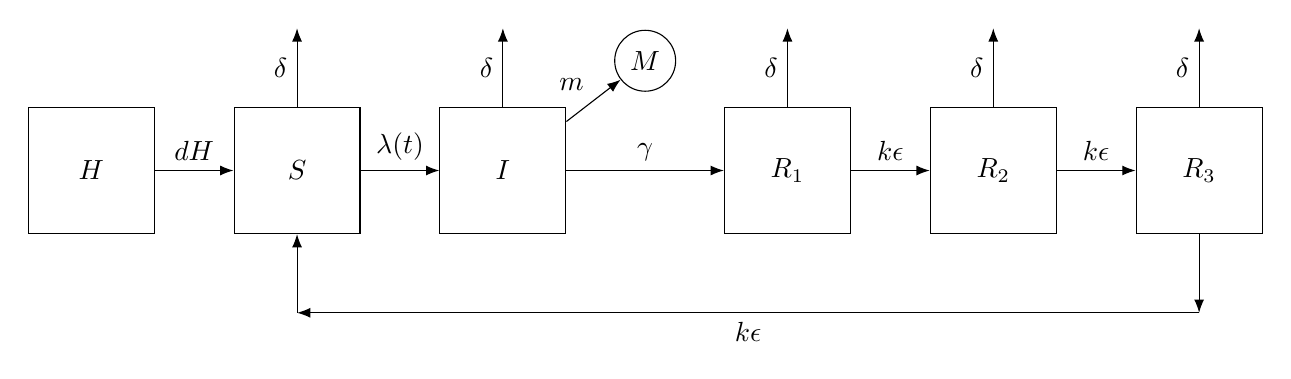
\begin{tikzpicture}[node distance=1cm and 1cm, auto,
>=Latex,every node/.append style={align=center}, 
int/.style={draw, minimum size=1.6cm}]
  \node [int] (H) at (0,0) {$H$};
\node [int] (S) [right=of H] {$S$};
\node [int] (I) [right=of S] {$I$};
\node (Mcoord) [right=of I, coordinate] {Mcoord};
\node [int] (R1) [right=of Mcoord] {$R_1$};
\node [int] (R2) [right=of R1] {$R_2$};
\node [int] (R3) [right=of R2] {$R_3$};
\node [circle, draw] (M) [above=of Mcoord] {$M$};
\node (deathsS) [above=of S, coordinate] {deathsS};
\node (deathsI) [above=of I, coordinate] {deathsS};
\node (deathsR1) [above=of R1, coordinate] {deathsR1};
\node (deathsR2) [above=of R2, coordinate] {deathsR2};
\node (deathsR3) [above=of R3, coordinate] {deathsR3};
\node (belowR3) [below=of R3, coordinate] {belowR3};
\node (belowS) [below=of S, coordinate] {belowS};
\path[->]
    (H) edge node {$dH$} (S)
    (S) edge node {$\lambda(t)$}  (I)
    (I) edge node {$\gamma$}  (R1)
    (R1) edge node {$k\epsilon$}  (R2)
    (R2) edge node {$k\epsilon$}  (R3)
    (R3) edge node {} (belowR3) 
    (belowR3) edge node {$k\epsilon$} (belowS) 
    (belowS) edge node {} (S)
    (I) edge node {$m$}  (M)
    (S) edge node {$\delta$}  (deathsS)
    (I) edge node {$\delta$}  (deathsI)
    (R1) edge node {$\delta$}  (deathsR1)
    (R2) edge node {$\delta$}  (deathsR2)
    (R3) edge node {$\delta$}  (deathsR3);
\end{tikzpicture}
\caption{Illustration of SIR model from \cite{king08}.}
\label{fig:sir}
\end{figure}

Figure \ref{fig:sir} depicts the above compartmental model that we use to benchmark the performance of IFAD. We present comparisons of IFAD with $\alpha=0$ (IFAD-0) and $\alpha=1$ (IFAD-1) against both (1) the results from \cite{ionides15}, and (2) our own implementation of IF2 in \texttt{JAX}. 

\paragraph{Hyperparameters:} While performing an initial exploratory analysis, we found that alternative hyperparameters for IF2 (random walk standard deviation of $\sigma=0.02$, geometrically decreasing cooling rate exponent $a=0.95$) performed better than the settings \cite{ionides15} chose, and chose to use these for our implementation to achieve a fairer comparison. Our implementations of IF2 and IFAD used 10000 particles, in line with \cite{ionides15}. 

\subsection{Results} 
We benchmarked IFAD against IF2 on a challenging global search problem. 100 initial starting parameter vectors were drawn uniformly from the same wide bounding box used in \cite{ionides15}, and we performed 100 searches each of IF2, IFAD-0.97, IFAD-0, and IFAD-1 initialized from these 100 starting parameter vectors. We summarize our findings below in Figures \ref{fig:scatter}, \ref{fig:boxplot-optim}, and \ref{fig:hist-all}. 


\begin{figure}[htbp!]
    \centering
    \includegraphics[scale=0.53]{../imgs/095/pairs.png}
    \includegraphics[scale=0.53]{../imgs/095/qq.png}
    \caption{Scatterplots depicting the performance of IFAD against that of IF2. \textbf{Left:} Paired searches from the same starting point. \textbf{Right:} Q-Q plot of ranked IFAD searches against ranked IF2 searches. It is clear that on average, IFAD has the edge, and manages to find the MLE while no IF2 search successfully gets within 7 log-likelihood units of it. We use a dotted red line to display the MLE in both. }

    \label{fig:scatter}
\end{figure}


\begin{figure}[htbp!]
    \centering
    \includegraphics[scale=0.5]{imgs/095/boxplot.png}
    \includegraphics[scale=0.5]{imgs/095/optim.png}
    \caption{\textbf{Left:} Results of best run out of every ten runs, simulating procedure of running a few searches and choosing the best one. IFAD outperforms IF2, and tuning $\alpha$ ultimately helps a lot. \textbf{Right:} Optimization plot of various methods. Solid lines depict the median negative log-likelihood at each iteration, while the shaded area depicts the best search at any iteration and the 80\% percentile.}
    \label{fig:boxplot-optim}
\end{figure}

\begin{figure}[htbp!]
    \centering
    \includegraphics[scale=0.35]{imgs/095/hist.png}
    \caption{Histogram comparison of IFAD, IF2, and MOP alone. Right is better.}
    \label{fig:hist-all}
\end{figure}

\subsection{Takeaways}

We obtain the following takeaways. IF2 converges quickly to a neighborhood of the MLE but fails to find the MLE. Gradient steps perform better at fine-grained refinement. In practice, we observe that performing gradient steps alone without a warm-start leads to the search getting stuck in local minima and saddle points. IFAD therefore combines the best of IF2 and MOP, approaching the MLE quickly and successfully performing refinement -- even on a very difficult global search problem.

\section{Discussion and Future Work}

We have developed a new theoretical framework, algorithm, and gradient estimator that encompasses the gradient estimates of \cite{blei2018vsmc} and \cite{poyiadjis11}. This yields a promising hybrid algorithm that warm-starts gradient descent (using this estimator) with IF2, that ultimately outperforms IF2 on Dhaka cholera model of \cite{king15}.

Still, there is yet quite a bit of work to do. Firstly, MOP-$\alpha$ cannot handle simulators that are not differentiable with the reparametrization trick. Working with likelihood ratios or straight-through gradient estimators may be potential ways to get around this. Secondly, the convergence rate of IF2 remains an open problem, and as such we do not know the convergence rate of the initial stage of IFAD -- only the gradient stage. Thirdly, here we have only explored the use of gradient descent for simplicity, even though other methods like Newton's method, ADAM, L-BFGS, etc. may perform better. Fourth, extensions to panel and spatiotemporal data, e.g. with a block particle filter in the lens of \cite{ionides22} and \cite{ning23}, are important for scientific applications. 


\bibliography{paper/bib-ifad,paper/bib-ref}
\bibliographystyle{apalike}

\appendix
\section{Lemmas for Correctness of MOP-$\alpha$}
\label{app:lemmas}
\begin{defn}[Targeting]
    A random vector $(X, w)$ drawn from a distribution $g$ \textbf{targets} the distribution $\pi$ if for any measurable and bounded functional $h$,
\begin{equation}
    E_g\{h(X) \cdot w\}=E_\pi\{h(X)\}
\end{equation}  
    A set of particles $(X^J_j, w^J_j), j=1,2, \ldots,J$, \textbf{targets} $\pi$ if for any measurable and bounded functional $h$,
\begin{equation}
    \frac{\sum_{j=1}^J h(X^J_j) w^J_j}{\sum_{j=1}^J w^J_j} \stackrel{a.s.}{\to} E_\pi(h(X))
\end{equation}
as $J \to \infty$.
\end{defn}


\begin{lem}[Change of Particle Measure]
    \label{lem:change-measure-proper-weights}
    Suppose that $\{(\tilde X_j^J,U_j^J),j=1,\dots,J\}$ targets $f_X$. Now, let $\{(Y_j^J,V_j^J),j=1,\dots,J\}$ be a multinomial sample drawn from $\{(\tilde X_j^J,U_j^J)\}$ where $(\tilde X_j^J,U_j^J)$ is represented, on average, proportional to $\pi^J_j J$ times. Write
    \[
    (Y_j^J,V_j^J) = \big(\tilde X^J_{a(j)},U^J_{a(j)}/\pi^J_{a(j)}\big),
    \]
    where $a$ is called the ancestor function. If the importance sampling weights $U_j/\pi_j$ are bounded, then $\{(Y^J_j,V^J_j),j=1,\dots,J\}$ targets $f_X$.
\end{lem}

\begin{proof}


    Note that as the $Y_j^J$ are a subsample from $X_j^J$, $h$ can be a function of $Y$ as well as it is one for $X$. We then expand
    $$\frac{\sum_j h(Y_j^J) V_j^J}{\sum_j V_j^J} = \frac{\sum_j h(\tilde X_{k_j}^J)\frac{U_{k_j}^J}{\pi_{k_j}^J}}{\sum_j \frac{U_{k_j}^J}{\pi_{k_j}^J}}.$$
    By hypothesis,
    $$\frac{\sum_j h(\tilde X_j^J)U_j^J}{\sum_j U_j^J} \stackrel{a.s.}{\to} \E_{f_X}[f(X)].$$

    We want to show
    \begin{equation}\label{eq:lemma1:h}
    \frac{\sum_j h(X_{k_j}^J)\frac{U_{k_j}^J}{\pi_{k_j}^J}}{\sum_j \frac{U_{k_j}^J}{\pi_{k_j}^J}} - \frac{\sum_j h(\tilde X_j^J)U_j^J}{\sum_j U_j^J} \stackrel{a.s.}{\to} 0.
    \end{equation}
    For this, it is sufficient to show that
   $$ \sum_j h(\tilde X_{k_j}^J)\frac{U_{k_j}^J}{\pi_{k_j}^J}
    -  \sum_j h(\tilde X_j^J)\frac{U_j^J}{\pi_j^J}\pi_j^J \stackrel{a.s.}{\to} 0 $$
    since an application of this result with $h(x)=1$ provides almost sure convergence of the denominator in (\ref{eq:lemma1:h}).
    Write $g(\tilde X_j^J) = h(\tilde X_j^J)\frac{U_{k_j}^J}{\pi_{k_j}^J}$. We therefore need to show that 
    $$\sum_j Z_j^J := \sum_j \left(g(\tilde X_{k_j}^J) -  g(\tilde X_j^J) \pi_j^J \right) \stackrel{a.s.}{\to} 0.$$

    Because the functional $h$ and importance sampling weights $u_{k_j}^J/\pi_{k_j}^J$ are bounded, we have that $\E[\left(Z_j^J\right)^4] < \infty$. We can then follow the argument of \cite{chopin20} from this point on, where 
    $$\E\left[\left(\sum_j Z_j^J\right)^4\right] 
    = J\E[(Z_1^J)^4] + 3J(J-1)\left(\E[(Z_j^J)^2]\right) \leq CJ^2,$$ for some $C>0$. By Markov, 
    $$\mathbb{P}\left(\left|\frac{1}{J} \sum_{j=1}^J Z_j^J\right|>\epsilon\right) 
    \leq \frac{1}{\epsilon^4J^4 } 
    \mathbb{E}\left[\left(\sum_{j=1}^J Z_j^J\right)^4\right] \leq \frac{C}{\epsilon^4J^2},$$
    and as these terms are summable we can apply Borel-Cantelli to conclude that these deviations happen only finitely often for every $\epsilon>0,$ giving us the almost-sure convergence for
    
    $$ \sum_j h(X_{k_j}^J)\frac{u_{k_j}^J}{\pi_{k_j}^J}
    -  \sum_j h(X_j^J)\frac{u_j^J}{\pi_j^J}\pi_j^J \stackrel{a.s.}{\to} 0.$$ 

    Similarly, we also have that
    $$ \sum_j \frac{u_j^J}{\pi_j^J}\pi_j^J
    - \sum_j \frac{u_{k_j}^J}{\pi_{k_j}^J} \stackrel{a.s.}{\to} 0,$$

    and the result is proved. 


    
    
   % Let $h$ be an integrable function. 
    %\begin{align*}
    %    \E\left[\sum_{j=1}^J h(Y_j) v_j\right] 
    %    &= \sum_{j=1}^J \E\left[h(X_{a(j)}) \frac{u_{a(j)}}{\pi_{a(j)}}\right] \\
    %    &= \sum_{j=1}^J \E\left[h(X_{j}) u_{j}\right],
    %\end{align*}
    %and similarly for the denominator. Now, the numerator and denominator of the reweighted quantity have the same expectation as the numerator and denominator of the original quantity, so they must converge to $ E_\pi(h(X))$ almost surely as well. 
\end{proof}


\textbf{Remark:} Note that Lemma \ref{lem:change-measure-proper-weights} permits $\pi_{1:J}$ to depend on $\{(X_j,u_j)\}$ as long as the resampling is carried out independently of $\{(X_j,u_j)\}$, conditional on $\pi_{1:J}$.

\begin{lem}[Particle Marginals]
    \label{lem:marginal-proper-weights}
    Suppose that $\{(\tilde X_j^J,U_j^J),j=1,\dots,J\}$ targets $f_X$. Also suppose that $\tilde Z_j^J \sim f_{Z|X}(\cdot | \tilde X_j^J)$ where $f_{Z|X}$ is a conditional probability density function corresponding to a joint density $f_{X,Z}$ with marginal densities $f_X$ and $f_Z$. Then, if the $U_j^J$ are bounded, $\{(\tilde Z_j^J,U_j^J)\}$ targets $f_Z$.
\end{lem}
\begin{proof}
    We want to show that, for any measurable bounded $h$, 
     $$\frac{\sum_j h(\tilde Z_j^J) \, U_j^J}{\sum_j U_j^J} \stackrel{a.s.}{\to} \E[h(Z)] = \E\big[\E[h(Z) | X]\big].$$
    By hypothesis, for any measurable and bounded functional $g$ with domain $\gX$,
    \begin{equation}\label{eq:lemma2:g}
    \frac{\sum_j g(\tilde X_j^J)\, U_j^J}{\sum_j U_j^J} \stackrel{a.s.}{\to} \E[g(X)].
    \end{equation}
    Let $\bar{U}_j^J = \frac{J U_j^J}{\sum_j U_j^J}$. Examine the numerator and denominator of the quantity $$\frac{J^{-1}\sum_j h(\tilde Z_j^J) \, U_j^J}{J^{-1}\sum_j U_j^J} = \frac{J^{-1}\sum_j h(\tilde Z_j^J) \, \bar{U}_j^J}{J^{-1}\sum_j \bar{U}_j^J}.$$
    The denominator converges to $1$ almost surely. The numerator, on the other hand, is
    $$\frac{1}{J}\sum_j h(\tilde Z_j^J)\, \bar{U}_j^J,$$
    by the same fourth moment argument to the above lemma converges almost surely to the limit of its expectation
    \begin{eqnarray*}        
    \lim_{J\to\infty} \E\left[\frac{1}{J}\sum_j h(\tilde Z_j^J)\, \bar{U}_j^J\right] 
    &=& \lim_{J\to\infty} \E \left[\frac{1}{J}\sum_j  
      \E\left[ h(\tilde Z_j^J)\, \bar{U}_j^J\big|\tilde X_j^J, \bar U_j^J\right]
    \right]
    \\
    &=& \lim_{J\to\infty} \E \left[\frac{1}{J}\sum_j  \E\big[h(Z) \big| X=\tilde X_j^J \big] \, \bar U_j^J\right].
    \end{eqnarray*}
    Applying (\ref{eq:lemma2:g}) with $g(x) = \E\big[h(Z) | X=x\big]$, the average on the right hand size converges almost surely to $\E\big\{\E[h(Z)|X]\big\}=\E[h(Z)].$
    It remains to swap the limit and expectations. We can do so with the bounded convergence theorem, and therefore obtain   
    $$\frac{1}{J}\sum_j h(\tilde Z_j^J)\,\bar{U}_j^J \stackrel{a.s.}{\to} \E[h(Z)].$$ 
    
\end{proof}

\begin{lem}[Particle Posteriors]
    \label{lem:posterior-proper-weights}
    Suppose that $\{(X_j^J,u_j^J),j=1,\dots,J\}$ targets $f_X$. Also suppose that $(X^{\prime J}_j,u^{\prime J}_j) = \big(X_j^J,u_j^J \cdot f_{Z|X}(z^*|X_j^J)\big)$. Then, if $u_j^J \cdot f_{Z|X}(z^*|X_j^J)\big)$ and $u_j^J \cdot f_{Z|X}(z^*|X_j^J)\big) / f_Z(z^*)$ are bounded, $\{(X^{\prime J}_j,u^{\prime J}_j)\}$ targets $f_{X|Z}(\cdot | z^*)$.
\end{lem}

\begin{proof}

        
    $$ \frac{J^{-1} \sum_j h(X_j^J) \bar{u}_j^{' J}}{J^{-1} \sum_j \bar{u}_j^{' J}}$$
    
    by
    
    \begin{equation}
    \frac{J^{-1} \sum_j h(X_j^J) f_{Z|X}(z^*|X_j^J) {u}_j^{J}}{J^{-1} \sum_j {u}_j^{J}}
    \times \left( \frac{J^{-1} \sum_j f_{Z|X}(z^*|X_j^J) {u}_j^{J}}{J^{-1} \sum_j {u}_j^{J}} \right)^{-1}
    \end{equation}
    

    Again, we want to show that
     $$\frac{\sum_j h(X_j^J) \cdot u_j^J \cdot f_{Z|X}(z^*|X_j^J)}{\sum_j u_j^J \cdot f_{Z|X}(z^*|X_j^J)} \stackrel{a.s.}{\to} \E_{f_{X|Z}}[h(X)|z^*].$$

    We already have that
    $$\frac{\sum_j h(X_j^J)u_j^J}{\sum_j u_j^J} \stackrel{a.s.}{\to} \E_{f_X}[h(X)].$$

    %= \frac{u_j^J \cdot f_{Z|X}(z^*|X_j^J)}{\sum_j f_{Z|X}(z^*|X_j^J)f_X(X_j^J)}

    Consider the following:
    \begin{equation}
    \frac{J^{-1} \sum_j h(X_j^J) f_{Z|X}(z^*|X_j^J) {u}_j^{J}}{J^{-1} \sum_j {u}_j^{J}}
    \times \left( \frac{J^{-1} \sum_j f_{Z|X}(z^*|X_j^J) {u}_j^{J}}{J^{-1} \sum_j {u}_j^{J}} \right)^{-1}.
    \end{equation}

    
    
    Write $\bar{u}_j^{J} = \frac{J u_j^J}{\sum_j u_j^J}$. Define the weights $u^{' J}_j := u_j^J \cdot f_{Z|X}(z^*|X_j^J),$ and the corresponding self-normalized weights $\bar{u}_j^{' J} := \frac{J u^{' J}_j}{\sum_j u^{' J}_j}.$ The denominator of the below quantity 
    $$ \frac{J^{-1} \sum_j h(X_j^J) \bar{u}_j^{' J}}{J^{-1} \sum_j \bar{u}_j^{' J}}$$
    converges to $1$, while the numerator, by the same fourth moment argument as the first lemma, converges almost surely to the limit of its expectation, which is
    \begin{align*}
        \lim_{J\to\infty} \E\left[J^{-1} \sum_j h(X_j^J) \bar{u}_j^{' J} \right]
        &= \lim_{J\to\infty} \E\left[J^{-1} \sum_j h(X_j^J) \frac{J u_j^J \cdot f_{Z|X}(z^*|X_j^J)}{\sum_j u_j^J \cdot f_{Z|X}(z^*|X_j^J)}\right] \\
        &= \lim_{J\to\infty} \E\left[J^{-1} \sum_j h(X_j^J) \frac{J \frac{u_j^J \cdot f_{Z|X}(z^*|X_j^J)}{f_Z(z^*)}}{\sum_j \frac{u_j^J \cdot f_{Z|X}(z^*|X_j^J)}{f_Z(z^*)}}\right]\\
        &= \lim_{J\to\infty} \E\left[ \sum_j h(X_j^J) \frac{\frac{u_j^J \cdot f_{Z|X}(z^*|X_j^J)}{f_Z(z^*)}}{\sum_j \frac{u_j^J \cdot f_{Z|X}(z^*|X_j^J)}{f_Z(z^*)}}\right]\\
        &= \E_{X|Z}[h(X)|z^*],
    \end{align*}

    where we can swap the limit and expectations with the bounded convergence theorem.
\end{proof}

\section{Variance Bound Proof}
\label{app:variance}

\subsection{Analysis of MOP-$\alpha$ Variance}

The proof strategy is as follows. Instead of analyzing the variance of the MOP-$\alpha$ gradient estimate proper, we will analyze the variance of a modified estimator where we truncate the weights at $k$ timesteps, so this estimator only looks at most $k$ timesteps back while accumulating the importance weights. This enables us to establish strong mixing for the truncated estimator, in order to get a bound on the variance that is $O(NJ^{-1})$. We emphasize that this estimator is only a theoretical construct -- we do not actually use this estimator. 

Coupled with a bound ensuring that the $k$-truncated estimator provides an estimate that is close to that of MOP-$\alpha$ proper, we get a bound on the variance of MOP-$\alpha$ that comprises of the variance of the $k$-truncated estimator plus the error, for any $k \leq N$. It then holds that the final variance bound on MOP-$\alpha$ is given by the minimum over all $k$, and is never larger than $O(1+NJ^{-1})$. 


Using the log-derivative trick and that $w_{n,j}^{F,\theta} = w_{n,j}^{F,\theta,k} = 1$ when $\theta=\phi$,
\begin{align*}
    &\left\lVert\nabla_\theta\log\left(\sum_{j=1}^J w_{n,j}^{F,\theta}\right)-\nabla_\theta\log\left(\sum_{j=1}^J w_{n,j}^{F,\theta,k}\right)\right\rVert_{\infty}\\
    &= \left\lVert\frac{\nabla_\theta\sum_{j=1}^J w_{n,j}^{F,\theta}}{{\sum_{j=1}^J w_{n,j}^{F,\theta}}}-\frac{\nabla_\theta\sum_{j=1}^J w_{n,j}^{F,\theta,k}}{{\sum_{j=1}^J w_{n,j}^{F,\theta,k}}}\right\rVert_{\infty} \\
    &= \left\lVert\frac{1}{J}\sum_{j=1}^J \nabla_\theta w_{n,j}^{F,\theta}-\frac{1}{J}\sum_{j=1}^J \nabla_\theta w_{n,j}^{F,\theta,k}\right\rVert_{\infty} \\
    &= \left\lVert\frac{1}{J}\sum_{j=1}^J \frac{\nabla_\theta w_{n,j}^{F,\theta}}{w_{n,j}^{F,\theta}}-\frac{1}{J}\sum_{j=1}^J \frac{\nabla_\theta w_{n,j}^{F,\theta,k}}{w_{n,j}^{F,\theta,k}}\right\rVert_{\infty} \\
    &= \left\lVert\frac{1}{J}\sum_{j=1}^J \nabla_\theta \log\left(w_{n,j}^{F,\theta}\right)-\frac{1}{J}\sum_{j=1}^J \nabla_\theta \log\left(w_{n,j}^{F,\theta,k}\right)\right\rVert_{\infty} \\
    &= \left\lVert\frac{1}{J}\sum_{j=1}^J \nabla_\theta \left(\log\left(w_{n,j}^{F,\theta}\right)-\log\left(w_{n,j}^{F,\theta,k}\right)\right)\right\rVert_{\infty}\\
    &= \left\lVert\frac{1}{J}\sum_{j=1}^J \nabla_\theta \left(\sum_{i=1}^n\alpha^{(n-i)}\log\left(\frac{g_{i,j}^{A,F,\theta}}{g_{i,j}^{A,F,\phi}} \right) - \sum_{i=n-k}^n{\alpha^{(n-i)}}\log\left(\frac{g_{i,j}^{A,F,\theta}}{g_{i,j}^{A,F,\phi}} \right)\right)\right\rVert_{\infty} \\
    &= \left\lVert\frac{1}{J}\sum_{j=1}^J \nabla_\theta \left(\sum_{i=1}^{n-k}\alpha^{(n-i)}\log\left(\frac{g_{i,j}^{A,F,\theta}}{g_{i,j}^{A,F,\phi}} \right) \right)\right\rVert_{\infty}\\
    &\leq \frac{1}{J}\sum_{j=1}^J \sum_{i=1}^{n-k}\alpha^{(n-i)}\left\lVert\nabla_\theta\log\left(g_{i,j}^{A,F,\theta} \right)\right\rVert_{\infty}\\
    &\leq \frac{1}{J}\sum_{j=1}^J \sum_{i=1}^{n-k}\alpha^{(n-i)}G'(\theta)\\
    &\leq G'(\theta)\frac{\alpha^k-\alpha^n}{1-\alpha},
\end{align*}
where the second-last line follows from Assumption \ref{assump:bounded-measurement}.


We can then bound $||\nabla_\theta\hat\ell(\theta) - \hat s_k(\theta)||$:
\begin{align*}
    &\left\lVert\nabla_\theta\hat\ell(\theta) - \hat s_k(\theta) \right\rVert_\infty\\
    &= \left\lVert\sum_{n=1}^N \nabla_\theta \log\left(\frac{\sum_{j=1}^J\prod_{i=1}^n\left(\frac{g_{i,j}^{A,F,\theta}}{g_{i,j}^{A,F,\phi}} \right)^{\alpha^{(n-i)}}}{\sum_{j=1}^J\prod_{i=1}^{n-1}\left(\frac{g_{i,j}^{A,F,\theta}}{g_{i,j}^{A,F,\phi}} \right)^{\alpha^{(n-i)}}}\right) - \sum_{n=1}^N \nabla_\theta\log\left(\frac{\sum_{j=1}^J\prod_{i=n-k}^n\left(\frac{g_{i,j}^{A,F,\theta}}{g_{i,j}^{A,F,\phi}} \right)^{\alpha^{(n-i)}}}{\sum_{j=1}^J\prod_{i=n-k}^{n-1}\left(\frac{g_{i,j}^{A,F,\theta}}{g_{i,j}^{A,F,\phi}} \right)^{\alpha^{(n-i)}}}\right) \right\rVert_\infty\\
    &= \Bigg\lVert\sum_{n=1}^N \nabla_\theta \Bigg(\log\left(\sum_{j=1}^J\prod_{i=1}^n\left(\frac{g_{i,j}^{A,F,\theta}}{g_{i,j}^{A,F,\phi}} \right)^{\alpha^{(n-i)}}\right)- \log\left(\sum_{j=1}^J\prod_{i=1}^{n-1}\left(\frac{g_{i,j}^{A,F,\theta}}{g_{i,j}^{A,F,\phi}} \right)^{\alpha^{(n-i)}}\right)\\
    &\qquad\qquad -\log\left(\sum_{j=1}^J\prod_{i=n-k}^n\left(\frac{g_{i,j}^{A,F,\theta}}{g_{i,j}^{A,F,\phi}} \right)^{\alpha^{(n-i)}}\right) + \log\left(\sum_{j=1}^J\prod_{i=n-k}^{n-1}\left(\frac{g_{i,j}^{A,F,\theta}}{g_{i,j}^{A,F,\phi}} \right)^{\alpha^{(n-i)}}\right)\Bigg)\Bigg\rVert_\infty \\
    &= \left\lVert\sum_{n=1}^N \nabla_\theta \Bigg(\log\left(\sum_{j=1}^Jw_{n,j}^{F,\theta}\right)- \log\left(\sum_{j=1}^Jw_{n,j}^{F,\theta,k}\right)
    -\log\left(\sum_{j=1}^Jw_{n-1,j}^{A, F,\theta}\right) + \log\left(\sum_{j=1}^Jw_{n-1,j}^{A, F,\theta,k}\right)\Bigg)\right\rVert_\infty \\
    &\leq \sum_{n=1}^N \left\lVert\nabla_\theta \left(\log\left(\sum_{j=1}^Jw_{n,j}^{F,\theta}\right)- \log\left(\sum_{j=1}^Jw_{n,j}^{F,\theta,k}\right)\right)\right\lVert_{\infty}
    +\sum_{n=1}^N \left\lVert\nabla_\theta \left(\log\left(\sum_{j=1}^Jw_{n-1,j}^{A, F,\theta}\right) + \log\left(\sum_{j=1}^Jw_{n-1,j}^{A, F,\theta,k}\right)\right)\right\rVert_\infty,
\end{align*}
and each of these two terms is bounded by $\frac{\alpha^k}{1-\alpha}NG'(\theta)$. So we now know that
$$\left\lVert\nabla_\theta\hat\ell(\theta) - \hat s_k(\theta) \right\rVert_\infty \leq  \frac{2\alpha^k}{1-\alpha}NG'(\theta),$$
which is our desired error bound. 

Now, we bound the variance of $\hat s_k(\theta)$. 
Recall that we defined
$$\hat s_k(\theta) = \sum_{n=1}^N \nabla_\theta\log\left(\frac{\sum_{j=1}^J\prod_{i=n-k}^n\left(\frac{g_{i,j}^{A,F,\theta}}{g_{i,j}^{A,F,\phi}} \right)^{\alpha^{(n-i)}}}{\sum_{j=1}^J\prod_{i=n-k}^{n-1}\left(\frac{g_{i,j}^{A,F,\theta}}{g_{i,j}^{A,F,\phi}} \right)^{\alpha^{(n-i)}}}\right) = \sum_{n=1}^N \nabla_\theta \left(\log\left(\sum_{j=1}^J w_{n,j}^{F,\theta, k}\right)-\log\left(\sum_{j=1}^J w_{n-1,j}^{A, F,\theta, k}\right)\right).$$

We can then decompose this expression with the log-derivative trick while noting that $w_{n,j}^{F,\theta, k} = 1$ whenever $\theta=\phi$, to see that
\begin{align*}
    \hat s_k(\theta) 
    &= \sum_{n=1}^N \nabla_\theta \left(\log\left(\sum_{j=1}^J w_{n,j}^{F,\theta, k}\right)-\log\left(\sum_{j=1}^J w_{n-1,j}^{A, F,\theta, k}\right)\right) \\
    &= \sum_{n=1}^N \left(\frac{\sum_{j=1}^J \nabla_\theta w_{n,j}^{F,\theta, k}}{\sum_{j=1}^J w_{n,j}^{F,\theta, k}}-\frac{\sum_{j=1}^J \nabla_\theta w_{n-1,j}^{A,F,\theta, k}}{\sum_{j=1}^J w_{n-1,j}^{A,F,\theta, k}}\right) \\
    &= \sum_{n=1}^N \left(\frac{1}{J}\sum_{j=1}^J \nabla_\theta w_{n,j}^{F,\theta, k}-\frac{1}{J}\sum_{j=1}^J \nabla_\theta w_{n-1,j}^{A,F,\theta, k}\right)\\
    &= \frac{1}{J}\sum_{n=1}^N \sum_{j=1}^J \nabla_\theta \left(w_{n,j}^{F,\theta, k}- w_{n-1,j}^{A,F,\theta, k}\right).
\end{align*}


It now follows that we need to bound the variance at a single timestep, namely
$$\text{Var}\left(\frac{1}{J}\sum_{j=1}^J\nabla_\theta \left(w_{n,j}^{F,\theta, k}- w_{n-1,j}^{A,F,\theta, k}\right)\right).$$

We use the log-derivative trick yet again to find, noting that $w_{n,j}^{F,\theta, k}=1$ when $\theta=\phi$, that
\begin{align*}
    \nabla_\theta w_{n,j}^{F,\theta, k} = \frac{\nabla_\theta w_{n,j}^{F,\theta, k}}{w_{n,j}^{F,\theta, k}} = \nabla_\theta \log(w_{n,j}^{F,\theta, k}) = \sum_{i=n-k}^n \alpha^{n-i} \nabla_\theta \log\left(\frac{g_{i,j}^{A,F,\theta}}{g_{i,j}^{A,F,\phi}} \right) = \sum_{i=n-k}^n \alpha^{n-i} \nabla_\theta \log\left(g_{i,j}^{A,F,\theta}\right).
\end{align*}

Then,
\begin{align*}
    \text{Var}\left(\nabla_\theta \left(w_{n,j}^{F,\theta, k}- w_{n-1,j}^{A,F,\theta, k}\right)\right) 
    &= \text{Var}\left(\nabla_\theta \left(\sum_{i=n-k}^n \alpha^{n-i} \nabla_\theta \log\left(g_{i,j}^{A,F,\theta}\right)- \sum_{i=n-k-1}^{n-1} \alpha^{n-i} \nabla_\theta \log\left(g_{i,j}^{A,F,\theta}\right)\right)\right) \\
    &= \text{Var} \left(\sum_{i=n-k}^n \nabla_\theta\left(\alpha^{n-i} \log\left(g_{i,j}^{A,F,\theta}\right)- \alpha^{n-i+1}\log\left(g_{i-1,j}^{A,F,\theta}\right)\right)\right).
\end{align*}


Note that $$\hat s_{n,k}(\theta) := \frac{1}{J}\sum_{j=1}^J\sum_{i=n-k}^n \nabla_\theta\left(\alpha^{n-i} \log\left(g_{i,j}^{A,F,\theta}\right)- \alpha^{n-i+1} \nabla_\theta \log\left(g_{i-1,j}^{A,F,\theta}\right)\right)$$ is a function bounded by $C\frac{G'(\theta)(1-\alpha^k)}{1-\alpha} =: CG'(\theta)r$ in each coordinate for some constant $C$ (by Assumption \ref{assump:bounded-measurement}) that depends only on $k$ timesteps, and not $n$. We can therefore invoke Lemma 2 of \cite{karjalainen2023} to bound the $L_2$ error of each of the $k$ (from time $n-k$ to time $n$) functionals from its expectation under the posterior by $CrG'(\theta)J^{-1/2}k$. That is, we have that
$$\E\left[||\hat s_{n,k}(\theta) - \E_{\pi}\hat s_{n,k}(\theta)||_\infty^2\right]^{1/2} \leq \frac{Cr^2G'(\theta) k}{\sqrt{J}}.$$


By the bias-variance decomposition, this in turn bounds the variance at a single timestep by $C^2r^2G'(\theta)^2J^{-1}k^2$. Concretely, we have that
$$\text{Var}\left(\frac{1}{J}\sum_{j=1}^J\sum_{i=n-k}^n \nabla_\theta\left(\alpha^{n-i} \log\left(g_{i,j}^{A,F,\theta}\right)- \alpha^{n-i+1} \log\left(g_{i-1,j}^{A,F,\theta}\right)\right)\right) \lesssim \frac{r^2k^2G'(\theta)^2}{J}.$$

It now remains to bound the variance of $\hat s_k(\theta)$ by considering the covariance of each of the $N$ terms that comprise it. We decompose
\begin{align*}
    \text{Var}(\nabla_\theta \hat s_k(\theta)) &= \text{Var}\left(\sum_{n=1}^N \frac{1}{J}\sum_{j=1}^J\sum_{i=n-k}^n \nabla_\theta\left(\alpha^{n-i} \log\left(g_{i,j}^{A,F,\theta}\right)- \alpha^{n-i+1} \log\left(g_{i-1,j}^{A,F,\theta}\right)\right)\right) \\
    &= \sum_{n=1}^N\text{Var}\left(\hat s_{n,k}(\theta)\right)+ 2\sum_{m<n}\text{Cov}\left(\hat s_{m,k}(\theta), \hat s_{n,k}(\theta)\right) \\
    &\lesssim \frac{r^2k^2G'(\theta)^2N}{J} + 2\sum_{m<n}\text{Cov}\left(\hat s_{m,k}(\theta), \hat s_{n,k}(\theta)\right).
\end{align*}

Similarly to the proof of the MOP-$0$ case, we use Assumptions \ref{assump:bounded-process} and \ref{assump:bounded-measurement} that ensure strong mixing. We know from Theorem 3 of \cite{karjalainen2023} that when $\textbf{M}_{n,n+k}$ is the $k$-step Markov operator from timestep $n$ and $\beta_{\text{TV}}(M) = \sup _{x, y \in E}\|M(x, \cdot)-M(y, \cdot)\|_{\mathrm{TV}}=\sup _{\mu, \nu \in \mathcal{P}, \mu \neq \nu} \frac{\|\mu M-\nu M\|_{\mathrm{TV}}}{\|\mu-\nu\|_{\mathrm{TV}}}$ is the Dobrushin contraction coefficient of a Markov operator, 
$$\beta_{\text{TV}}(\textbf{M}_{n,n+k}) \leq (1-\epsilon)^{\floor{k/(c\log(J))}},$$
i.e. the mixing time of the particle filter is $O(\log(J))$, where $\epsilon$ and $c$ depend on $\bar{M}, \underbar{M}, \bar{G}, \underbar{G}$ in \ref{assump:bounded-process} and \ref{assump:bounded-measurement}. By Lemma \ref{lem:dobrushin-implies-alpha-mixing}, the particle filter itself is strongly mixing, with $\alpha$-mixing coefficients $\alpha(l) \leq (1-\epsilon)^{\floor{l/(c\log(J))}}$. Therefore, functions of particles are strongly mixing as well, with $\alpha$-mixing coefficients bounded by the original (to see this, observe that the $\sigma$-algebra of the functionals is contained within the original $\sigma$-algebra).

We now derive the $\alpha$-mixing coefficients of $(\hat s_{n,k}(\theta))_{n=1}^N$. Observe that $\hat s_{n,k}$ is strong mixing at lag $k+1$, as all weights beyond $k$ timesteps are truncated. We therefore have that the mixing time of $\hat s_k(\theta)$ is $O(1+k+\log(J))$, and that the $\alpha$-mixing coefficients for $(\hat s_{n,k}(\theta))_{n=1}^N$ are given by $\alpha(l) \leq (1-\epsilon)^{\floor{l/(c(1+k+\log(J)))}}$.

Therefore, by Davydov's inequality and Lemma 2 of \cite{karjalainen2023}, and noting that $\hat s_{n,k}(\theta) \leq CrG'(\theta)$ by Assumption \ref{assump:bounded-measurement}, by a similar argument to the MOP-0 case, we find that 

$$\text{Cov}\left(\hat s_{m,k}(\theta), \hat s_{n,k}(\theta)\right) \lesssim (1-\epsilon)^{\frac{1}{2}\floor{\frac{|n-m|}{c(1+k+\log(J))}}}\frac{r^2G'(\theta)^2}{J}.$$

Concretely, noting that $\nabla_\theta\hat s_{n,k}(\theta)\leq CrG'(\theta)$ by Assumption \ref{assump:bounded-measurement}, and WLOG assuming $\E[(\nabla_\theta\hat\hat s_{m,k}(\theta))^4]^{1/4}\leq\E[(\nabla_\theta\hat\hat s_{n,k}(\theta))^4]^{1/4}$, we apply Davydov's inequality to see that
\begin{align*}
    \text{Cov}(\nabla_\theta\hat s_{m,k}(\theta), \nabla_\theta\hat s_{n,k}(\theta)) 
    &\leq \alpha(n-m)^{1/2}\E[(\nabla_\theta\hat s_{m,k}(\theta))^4]^{1/4}\E[(\nabla_\theta\hat s_{n,k}(\theta))^4]^{1/4}\\
    &\leq \alpha(n-m)^{1/2}\E[(\nabla_\theta\hat s_{n,k}(\theta))^4]^{1/2}.
\end{align*}

To bound this, we use the fact that $$\E[(\nabla_\theta\hat s_{n,k}(\theta))^4] = \E[(\nabla_\theta\hat s_{n,k}(\theta)-\E[\nabla_\theta\hat s_{n,k}(\theta)])^4]+\E[(\nabla_\theta\hat s_{n,k}(\theta))^2]^2$$
alongside Lemma 2 of \cite{karjalainen2023}, which shows that
$$\E[(\nabla_\theta\hat s_{n,k}(\theta)-\E[\nabla_\theta\hat s_{n,k}(\theta)])^4] \lesssim \frac{r^4G'(\theta)^4}{J^2}, \;\; \E[(\nabla_\theta\hat s_{n,k}(\theta)-\E[\nabla_\theta\hat s_{n,k}(\theta)])^2] \lesssim \frac{r^2G'(\theta)^2}{J},$$
to find that 
$$\E[(\nabla_\theta\hat s_{n,k}(\theta))^4]^{1/2} \lesssim  \sqrt{\frac{r^4G'(\theta)^4}{J^2}+\left(\frac{r^2G'(\theta)^2}{J}\right)^2} = \frac{r^2G'(\theta)^2}{J},$$
and conclude that 
$$\text{Cov}(\nabla_\theta\hat s_{m,k}(\theta), \nabla_\theta\hat s_{n,k}(\theta)) \leq (1-\epsilon)^{\frac{1}{2}\floor{\frac{|n-m|}{c(1+k+\log(J))}}}\frac{r^2G'(\theta)^2}{J}.$$


Putting it all together, we see that
\begin{align*}
    \text{Var}(\nabla_\theta \hat s_{k}(\theta)) &= \sum_{n=1}^N \text{Var}(\nabla_\theta\hat s_{n,k}(\theta)) + 2\sum_{m<n} \text{Cov}(\nabla_\theta\hat s_{m,k}(\theta),\nabla_\theta\hat s_{n,k}(\theta))\\
    &\leq \frac{Nr^2k^2G'(\theta)^2}{J} + 2\sum_{n=1}^{N-1} (N-n)(1-\epsilon)^{\frac{1}{2}\floor{\frac{n}{c(1+k+\log(J))}}}\frac{r^2G'(\theta)^2}{J} \\
    &\leq \frac{r^2k^2G'(\theta)^2}{J} \left(N + 2\sum_{n=1}^{N-1} (N-n) (1-\epsilon)^{\frac{1}{2}\floor{\frac{n}{c(1+k+\log(J))}}}\right) \\
    &\lesssim \frac{k^2r^2G'(\theta)^2N}{J}.
\end{align*}

We will now use this result to bound $\text{Var}(\nabla_\theta \hat s_k(\theta)$ proper. For random variables $X,Y$ where $|X-Y|$ is bounded almost surely by some $M$, we have that 
$$X-\E X - 2M \leq Y - \E Y \leq X - \E X + 2M$$
so,
$$(Y-\E Y)^2 \leq (X-\E X - 2M)^2 + (X-\E X +2M)^2.$$
Taking expectations, we get
$$\text{Var}(Y) \leq \text{Var}(X) + 8M^2.$$

It follows from this result and the result we proved earlier, namely that
$$||\nabla_\theta\hat\ell(\theta) - \hat s_k(\theta)||_\infty \leq \frac{2\alpha^k}{1-\alpha}NG'(\theta),$$
that the variance of MOP-$\alpha$ proper is bounded by, for any $k \leq N$,
that the variance of MOP-$\alpha$ proper is bounded by
$$\text{Var}(\nabla_\theta \hat\ell(\theta)) \lesssim \frac{k^2r^2G'(\theta)^2N}{J} + \frac{16\alpha^{2k}}{(1-\alpha)^2}N^2G'(\theta)^2.$$

As the above holds for any $k \leq N$,
$$\text{Var}(\nabla_\theta \hat\ell(\theta)) \lesssim \min_{k\leq N} \left(\frac{k^2G'(\theta)^2N}{(1-\alpha)^2J} + \frac{16\alpha^{2k}}{(1-\alpha)^2}N^2G'(\theta)^2 \right).$$

Note that the result here is presented in the sup norm. In the main text, we provide the result in the $2$-norm, and therefore scale the above result by $p$. 


\end{document}
